%%%%%%%%%%%%%%%%%%%%%%%%%%%%%%%%%%%%%%%%%%%%%%%%%%%%%%%%%%%%%%%%%%%%%
%% This is a (brief) model paper using the achemso class
%% The document class accepts keyval options, which should include
%% the target journal and optionally the manuscript type. 
%%%%%%%%%%%%%%%%%%%%%%%%%%%%%%%%%%%%%%%%%%%%%%%%%%%%%%%%%%%%%%%%%%%%%
\documentclass[journal=jcisd8,manuscript=article]{achemso}

%%%%%%%%%%%%%%%%%%%%%%%%%%%%%%%%%%%%%%%%%%%%%%%%%%%%%%%%%%%%%%%%%%%%%
%% Place any additional packages needed here.  Only include packages
%% which are essential, to avoid problems later. Do NOT use any
%% packages which require e-TeX (for example etoolbox): the e-TeX
%% extensions are not currently available on the ACS conversion
%% servers.
%%%%%%%%%%%%%%%%%%%%%%%%%%%%%%%%%%%%%%%%%%%%%%%%%%%%%%%%%%%%%%%%%%%%%
\usepackage[version=3]{mhchem} % Formula subscripts using \ce{}
\usepackage{graphicx}
\usepackage{subcaption}
\usepackage{array}
\usepackage{url}
\usepackage{hyperref}
\usepackage{xr-hyper}
\usepackage{multirow}
\usepackage{listings}

%%%%%%%%%%%%%%%%%%%%%%%%%%%%%%%%%%%%%%%%%%%%%%%%%%%%%%%%%%%%%%%%%%%%%
%% If issues arise when submitting your manuscript, you may want to
%% un-comment the next line.  This provides information on the
%% version of every file you have used.
%%%%%%%%%%%%%%%%%%%%%%%%%%%%%%%%%%%%%%%%%%%%%%%%%%%%%%%%%%%%%%%%%%%%%
%%\listfiles

%%%%%%%%%%%%%%%%%%%%%%%%%%%%%%%%%%%%%%%%%%%%%%%%%%%%%%%%%%%%%%%%%%%%%
%% Place any additional macros here.  Please use \newcommand* where
%% possible, and avoid layout-changing macros (which are not used
%% when typesetting).
%%%%%%%%%%%%%%%%%%%%%%%%%%%%%%%%%%%%%%%%%%%%%%%%%%%%%%%%%%%%%%%%%%%%%
\lstset{%
breaklines=true,
breakatwhitespace=true,
captionpos=b,
frame=single
}
\newcommand*\mycommand[1]{\texttt{\emph{#1}}}
\makeatletter
\newcommand*{\addFileDependency}[1]{% argument=file name and extension
  \typeout{(#1)}
  \@addtofilelist{#1}
  \IfFileExists{#1}{}{\typeout{No file #1.}}
}
\newcommand*{\myexternaldocument}[1]{%
    \externaldocument{#1}%
    \addFileDependency{#1.tex}%
    \addFileDependency{#1.aux}%
}
\makeatother
\myexternaldocument{supplement}


\author{Andrew McNutt}
\author{Paul Francoeur}
\affiliation[University of Pittsburgh]
{Department of Computational and Systems Biology, University of Pittsburgh, Pittsburgh, PA}
\author{Rishal Aggarwal}
\affiliation[International Institute of Information Technology Hyderabad]
{Center for Computational Natural Sciences and Bioinformatics, International Institute of Information Technology, Hyderabad 500 032, India}
\author{Tomohide Masuda}
\affiliation[University of Pittsburgh]
{Department of Computational and Systems Biology, University of Pittsburgh, Pittsburgh, PA}
\author{Rocco Meli}
\affiliation[University of Oxford]{Department of Biochemistry, University of Oxford, Oxford, United Kingdom}
\author{Matthew Ragoza}
\author{Jocelyn Sunseri}
\author{David Ryan Koes}
\email{dkoes@pitt.edu}
\affiliation[University of Pittsburgh]
{Department of Computational and Systems Biology, University of Pittsburgh, Pittsburgh, PA}


%%%%%%%%%%%%%%%%%%%%%%%%%%%%%%%%%%%%%%%%%%%%%%%%%%%%%%%%%%%%%%%%%%%%%
%% The document title should be given as usual. Some journals require
%% a running title from the author: this should be supplied as an
%% optional argument to \title.
%%%%%%%%%%%%%%%%%%%%%%%%%%%%%%%%%%%%%%%%%%%%%%%%%%%%%%%%%%%%%%%%%%%%%
\title[GNINA 1.0]
  {GNINA 1.0: Molecular docking with deep learning}

%%%%%%%%%%%%%%%%%%%%%%%%%%%%%%%%%%%%%%%%%%%%%%%%%%%%%%%%%%%%%%%%%%%%%
%% Some journals require a list of abbreviations or keywords to be
%% supplied. These should be set up here, and will be printed after
%% the title and author information, if needed.
%%%%%%%%%%%%%%%%%%%%%%%%%%%%%%%%%%%%%%%%%%%%%%%%%%%%%%%%%%%%%%%%%%%%%
\keywords{molecular docking, deep learning, structure-based drug design}

%%%%%%%%%%%%%%%%%%%%%%%%%%%%%%%%%%%%%%%%%%%%%%%%%%%%%%%%%%%%%%%%%%%%%
%% The manuscript does not need to include \maketitle, which is
%% executed automatically.
%%%%%%%%%%%%%%%%%%%%%%%%%%%%%%%%%%%%%%%%%%%%%%%%%%%%%%%%%%%%%%%%%%%%%
\begin{document}

%%%%%%%%%%%%%%%%%%%%%%%%%%%%%%%%%%%%%%%%%%%%%%%%%%%%%%%%%%%%%%%%%%%%%
%% The "tocentry" environment can be used to create an entry for the
%% graphical table of contents. It is given here as some journals
%% require that it is printed as part of the abstract page. It will
%% be automatically moved as appropriate.
%%%%%%%%%%%%%%%%%%%%%%%%%%%%%%%%%%%%%%%%%%%%%%%%%%%%%%%%%%%%%%%%%%%%%
\begin{tocentry}

\end{tocentry}

%%%%%%%%%%%%%%%%%%%%%%%%%%%%%%%%%%%%%%%%%%%%%%%%%%%%%%%%%%%%%%%%%%%%%
%% The abstract environment will automatically gobble the contents
%% if an abstract is not used by the target journal.
%%%%%%%%%%%%%%%%%%%%%%%%%%%%%%%%%%%%%%%%%%%%%%%%%%%%%%%%%%%%%%%%%%%%%
\begin{abstract}

\end{abstract}


%%%%%%%%%%%%%%%%%%%%%%%%%%%%%%%%%%%%%%%%%%%%%%%%%%%%%%%%%%%%%%%%%%%%%
%% Start the main part of the manuscript here.
%%%%%%%%%%%%%%%%%%%%%%%%%%%%%%%%%%%%%%%%%%%%%%%%%%%%%%%%%%%%%%%%%%%%%
\section{Introduction}

Molecular docking is a computational procedure in which the non-covalent bonding of molecules is predicted, most often a protein receptor and a ligand. Docking predicts the binding affinity and conformation of the small molecule in its minimal energy state and is used to virtually screen large libraries of compounds\cite{kitchen2004docking,leach2006prediction,lyu2019ultra}. Docking is composed of two main steps, sampling and scoring. Sampling refers to an extensive search of the conformational space of the molecule being docked. Proper sampling requires thorough coverage of the conformational landscape of both the ligand and the protein. The flexibility of the ligand and the protein determine the conformations that can be accessed, expanding the search space when flexibility of either molecule is increased. The other vital piece of a molecular docking software is the scoring function. Every pose sampled by the algorithm is evaluated for its fitness in comparison to other conformations. The scoring function determines the conformations that are retained from the sampling of the search space and ranks the retained poses in order of their likelihood of being correct. The final output is a set of ranked poses of the docked molecule that are then assigned a binding affinity. Determination of the correct binding pose of the small molecule allows us to properly determine the binding affinity of the molecule and affords the opportunity to utilize the pose for lead optimization of the small molecule. Correct evaluation of binding affinity is critical for downstream tasks such as virtual screening or for determining if a compound is important for more experimental analysis. Molecular docking must provide a pose and a binding affinity quickly for it to aid the drug discovery pipeline. Sampling the entire conformational space of a molecule is not a quick task, therefore, we compromise on the speed and accuracy of docking to provide poses that are close to native while not requiring the full search of conformational space. This compromise requires docking software to focus on the accuracy and ranking power of the scoring function to highlight low energy conformations and reduce extraneous sampling.

Scoring functions provide a mapping from the conformational space of the ligand and receptor to a real number so that poses may be ranked. Typically, scoring functions are grouped into three categories; knowledge based, physics based, and empirical \cite{kitchen2004docking}. Knowledge based scoring functions leverage the statistics from a set of structural binding data. A number of properties are computed from structures of protein-ligand complexes, such as atom-atom pairwise contacts. The calculated frequencies can be used in a method such as Potential Mean Force, which creates a potential based on the Boltzmann distribution of the properties, to calculate the score of a pose. Knowledge based scoring functions tend to generalize well and calculations of scores are quick at test time. However, they require a large database of known structures, largely ignore the effect of solvents, and can be difficult to interpret when trying to understand a score\cite{brooijmans2003molecular}. Physics based scoring functions, often referred to as force fields, utilize physically derived energetics of interactions to compute scores. The final score is a combination of energy terms such as Coulombic and van der Waals forces\cite{huang2006molecular}. Accuracy of physics based scoring functions are limited by understanding of fundamental forces dictating interactions between molecules, though understanding of these forces is continually increasing\cite{liu2015classification}. Empirical scoring functions address the limitations of physics based scoring functions by weighting the individual force terms to fit to experimental data.  A large proportion of docking software use empirical scoring functions, including X-score, Autodock Vina, and ChemScore\cite{wang2002further,trott2010autodock,eldridge1997empirical}. Unlike knowledge based scoring functions, empirical scoring functions allow simple interpretation of what is contributing to the score. Fitting the scoring function requires lots of experimental structural data and prevents the combination of terms from separate scoring functions. These categories of scoring functions are limited to features extracted from structural information with the assumption that there is a linear relationship between the features and the binding affinity. Autodock Vina (called `Vina') utilizes an empirical scoring function explicitly tuned to structural data\cite{trott2010autodock}. The scoring function is a weighted sum of atomic interactions.  Steric, hydrophobic, and hydrogen bonding interactions are calculated and are adjusted by the number of rotatable bonds to account for entropic penalties. The weights of the terms being denoted by a non-linear fit to structural data. \citet{nguyen2019autodock} show that Vina can more accurately predict the binding pose than its predecessor, Autodock 4\cite{morris1998automated}. With the success of Vina, over its predecessor, we search for alternative scoring functions that are able to model non-linear relationships and automatically extract features from structural information without explicit featurization.

Machine learning(ML) algorithms learn arbitrary relationships between observations and outputs. There has been considerable progress in other biomedical fields with the utilization of ML models\cite{zitnik2019machine}. However, machine learning algorithms require a large amount of data to properly generalize to unseen information. The last 20 years has seen a noteworthy increase in the quantity of available protein structures\cite{berman2000protein}. A plethora of databases annotate structural data with experimental binding affinity data, including PDBBind and BindingDB\cite{wang2004pdbbind,liu2017forging,gilson2016bindingdb}. This information has been utilized to leverage machine learning algorithms as scoring functions. A number of traditional ML approaches have been used as scoring functions, including random forests (RF-Score\cite{ballester2010machine} and SFCScore\cite{zilian2013sfcscore}), support vector machines (SVR-SF\cite{li2011svr}, ID-Score\cite{li2013idscore}, SVR-EP), artificial neural networks (NNscore\cite{durrant2010nnscore} and BsN-Score\cite{ashtawy2015bsn}), and gradient boosted decision trees (BT-dock\cite{btdock} and ESPH T-Bind\cite{cang2018integration}). These ML methods have been able to match or exceed existing traditional scoring functions. ML methods allow a more robust fit to the training data, but are limited to the features explicitly extracted from structural data.

Deep Learning (DL) methods allow direct inference of features from inputs. These methods have demonstrated success in a variety of fields, such as computer vision and natural language processing\cite{krizhevsky2017imagenet,brown2020language}. In recent years, there has been significant progress with DL methods in the drug discovery field with many models employing a convolutional framework. Convolutional Neural Networks(CNN) leverage convolutions to infer features directly from input tensors, usually images. CNNs have shown potential in virtual screening (AtomNet\cite{wallach2015atomnet}, DeepVS\cite{pereira2016boosting}, Ragoza et al.\cite{Ragoza2017}) and binding affinity prediction (PotentialNet\cite{feinberg2018potentialnet}, $K_{DEEP}$\cite{jimenez2018k}, Pafnucy\cite{stepniewska2018development}). A number of methods have been proposed to capitalize on the power of DL scoring functions. MedusaNet uses a CNN within the docking pipeline to guide the sampling of the base docking method\cite{jiang2020guiding}. The base docking method, Medusa, provides a variety of ligand poses that are translated to a 3D coordinate representation which the CNN evaluates for determination of whether to keep the pose. Nguyen et al. \cite{nguyen2020mathdl} describe a generative adversarial network (GAN) for pose prediction. Their network utilizes an encoder with low-dimensional mathematical representations of the protein-ligand complex and a decoder utilizing convolutional layers to generate and rank ligand poses for the D3R grand challenge. Masuda et al. \cite{masuda2020generating} use a receptor structure as the prior to their GAN to simultaneously sample and score novel ligands.

In this work, we describe and comprehensively evaluate version 1.0 of the \textsc{Gnina} molecular docking software, a fork of \textsc{Smina}\cite{koes2013lessons} and Vina\cite{trott2010autodock} that supports CNN scoring as an integral part of the docking workflow. We describe how default settings that balance docking accuracy and run-time performance were determined, including the selection of a default ensemble of CNN models. Performance of \textsc{GNINA} is evaluated for the redocking, cross-docking, flexible docking, and whole protein docking tasks and is found to significantly outperform \textsc{Smina}/Vina in all cases.



\section{Methods}

The docking pipeline of \textsc{Gnina} is described in detail, providing background for the derivation of default usage. A default CNN ensemble is selected for optimizing the docking performance and run-time of the docking pipeline. This ensemble is then used to investigate the different CNN scoring options available to the user, followed by a thorough investigation of the docking arguments. Finally, we examine the settings for both generalizability and scoring power.

\subsection{Molecular Docking Pipeline}
\textsc{\textsc{Gnina}} is a fork of \textsc{Smina}\cite{koes2013lessons} which is a fork of Vina\cite{trott2010autodock}. The docking pipeline of \textsc{\textsc{Gnina}} utilizes the enhanced support for scoring enabled in \textsc{Smina} to allow the use of CNNs as scoring functions. In typical usage, \textsc{\textsc{Gnina}} is provided with a receptor structure, a ligand structure, and a specification for a binding site on the receptor(\texttt{autobox\_ligand}).
\begin{lstlisting}[title=Example Gnina Usage,label=code:Usage,language=bash]
    gnina --receptor 1BCU_PROT.pdb --ligand 1BCU_LIG.sdf --out 1BCU_gnina_poses.sdf.gz --autobox_ligand 1BCU_LIG.sdf --autobox_add 4 --cnn Crossdock_Default2018 Dense_3 --cnn_scoring rescore --exhaustiveness 8 --num_mc_saved 50 --cnn_rotation 0 --num_modes 9 --min_rmsd_filter 1
\end{lstlisting}
Open Babel\cite{o2011open,babelopen}, a chemical toolbox allowing the reading and writing of over 100 chemical file formats, is used for parsing the inputs, allowing commonly used structural data formats (i.e. PDB, sdf, mol, etc.) to be used as input. The binding site can be specified as a Cartesian box or by providing an ``autobox'' ligand.  When a ligand is used to define the binding site, a box is defined using the minimum and maximum values for the $x$, $y$, and $z$ coordinates of the ligand to define a rectangular prism to which additional spacing (\texttt{autobox\_add}) is added in every dimension. In \textsc{Gnina}, if any side of this auto-generated box is smaller than the longest distance between any two atoms in the ligand, then those sides are extended to that longest distance, ensuring that the ligand can rotate freely within the defined box without incurring an out-of-box penalty that is applied to all dock poses to constrain them to the specified binding site search space.

Next the scoring functions are setup. Similar to \textsc{Smina}, the user can specify their own empirical scoring function to \textsc{Gnina} or use one of the built-in scoring functions, i.e. Vina, Vinardo\cite{quiroga2016vinardo}, etc. CNN scoring functions can be specified by providing model and/or weights files or by selecting a built-in model.  The available built-in CNN models include Crossdock\_Default2018, Dense, General\_Default2018, Redock\_Default2018, and Default2017. Each of these CNN models, excluding Default2017, has five variants which are trained on the same data and have the same architecture, but are initialized with a different random seed. For each CNN model type, we refer to the variant with the highest docking performance as the base model name, and the remaining variants are given sequential numbers (i.e. General\_Default2018, General\_Default2018\_1, General\_Default2018\_2, General\_Default2018\_3, and General\_Default2018\_4); the ensemble of these five variants is denoted with `Ensemble' (i.e. General\_Default2018 Ensemble). The architecture and training of these models are described elsewhere \cite{francoeur2020three,Ragoza2017}. These models are trained to predict both a pose score (a probability that the pose is a low-RMSD pose) and the binding affinity (pK).  For all pose optimization tasks the pose score is used.

The docking procedure is a Monte Carlo sampling method. \texttt{exhaustiveness} (default 8) defines the number of Monte Carlo chains that are run for the ligand. The number of steps for the Monte Carlo chains are calculated based on the number of mobile atoms and the number of degrees of freedom within the ligand. Each Monte Carlo chain randomly mutates the ligand by randomly selecting one of the following operations: random translation, random rotation of the entire molecule, or randomly setting the torsional angles of the ligand. The mutation favors the random resetting of the torsional angles over the other mutations. After the mutation, a quick energy minimization of the ligand is performed.  If an empirical scoring function is specified for guiding sampling, this minimization is performed using a fast, grid-based approximation of that scoring function.  A grid is pre-calculated for each ligand atom type and single atom probes are used to calculate values for each grid point.  The full ligand is scored by interpolating values from the grid for each of its atoms and summing the result.  If a CNN scoring function is specified, no such approximation is used since CNN scoring is not additive with respect to the individual atoms\cite{hochuli2018visualizing}.
 The score for the minimized conformation determines if it will be accepted using the Metropolis acceptance criterion. Each Monte Carlo chain retains its top scoring  ligand conformations, and the number retained is user configurable with \texttt{num\_mc\_saved}(default 50).

Following the completion of Monte Carlo sampling, the saved conformations from each Monte Carlo chain are pooled and the top scoring conformations are retained for further analysis. The top scoring conformations are then refined. If an empirical scoring function is specified for refinement, then the fast grid approximation is not used in order to get the best possible locally optimal pose. After the ligand pose has been refined, the final affinities and scores are calculated for the pose using the specified CNN models and/or the specified scoring function. Finally, the top scoring conformations are sorted based on one of the scores, determined by the user (default CNNscore), and output with Open Babel in the user specified format if an output file was provided.


The usage of the CNN models within the docking pipeline can be selected by the user using \texttt{cnn\_scoring}. If ``none'' is selected for \texttt{cnn\_scoring}, then the CNN models are not used at all in the docking pipeline, making the pipeline essentially identical to the \textsc{Smina} pipeline. When ``rescoring'' is selected (the default), the specified CNN models are not used until the final sorting of the refined ligand conformations. The specified CNN models are used to score each of the ligand conformations and the output ligand conformations are resorted based on the score calculated by the CNN model(s). The ``refinement'' option utilizes the CNN for the refinement of the ligand poses after they have been selected by the Monte Carlo chains and then sorts the refined ligand conformations by the CNN score for output. Finally, the ``all'' option utilizes the CNN for all aspects of the docking pipeline including the minimization within the Monte Carlo chains, the refinement after the Monte Carlo chains, and the sorting of the final output. 

\subsubsection{Flexible Docking}

Molecular docking is often performed using a rigid protein target and only the conformational space of the ligand is sampled, as described above. This is a good approximation when redocking to a receptor that is mostly rigid, but it breaks down when the protein undergoes significant structural changes upon complexation\cite{Teague2003}. While whole target relaxation is too computationally expensive for docking, some protein flexibility can be accounted for by sampling the conformational space of side chains in the binding site\cite{Zhao2008}. The local flexibility of the binding site could be especially beneficial for cross-docking, where the assumption of a rigid receptor is not realistic when potentially very different ligands are docked to the same receptor.

GNINA allows the sampling of side chain, but not backbone, conformational space, on the same footing of the ligand conformational space. The side chains to be treated as flexible can be specified manually or semi-automatically in different ways: they can be specified in a PDBQT file (\texttt{flex} parameter), they can be selected using a comma-separated list of residue identifiers (chain, residue number, and, optionally, insertion code; \texttt{flexres} parameter) or they can be selected based on their distance from a given ligand (\texttt{flexdist} and \texttt{flexdist\_ligand} parameters) similarly to the \texttt{autobox\_ligand} option described above. For the latter method, used in this work, \texttt{flexdist} specifies a distance from \texttt{flexdist\_ligand}. If a side chain has any atoms that are within this distance of the specified ligand, then it is marked as flexible. 

Given the increased computational time of sampling side chains' conformations, two additional options are provided. \texttt{flex\_limit} allows to specify a hard upper bound for the number of flexible side chains included, over which the calculation does not run. The less strict \texttt{flex\_max} allows to prune the list of flexible side chains by specifying the maximum number of them that can be included in the calculation (closest to \texttt{flexdist\_ligand}).

Flexible side chains are selected at the very beginning and the selection is not updated during docking. When using \texttt{autobox} to automatically define the search space as described above, flexible side chains are included in the calculation of the box bounds.

The usage of CNN models for docking with flexible side chains can be selected by the user in the same way it is done for docking with a rigid receptor, as described above.

\subsection{Data}
There are two primary ways to evaluate molecular docking: redocking a cognate ligand to its receptor and docking a ligand to a non-cognate receptor (cross-docking). In order to best evaluate the performance of \textsc{Gnina} for molecular docking we evaluate its performance on both of these tasks. Redocking the cognate ligand easily demonstrates the sampling and scoring power of the molecular docking pipeline, as the root mean square deviation (RMSD) from the crystal pose can be measured to exactly determine the accuracy of the produced poses. Analysis of redocking requires a set of high quality structures in which the native binding pose of the ligand has been solved. For this purpose we utilize the PDBbind refined set v.2019\cite{liu2017forging}. The PDBBind database is a curated set of protein ligand binding information containing both structural information and binding affinity. The PDBBind database is updated annually with new experimentally determined structures annotated with binding affinity data. The refined set is a subset of the entire PDBbind dataset that filters the structures with resolution higher than 2.5 \AA, high quality affinity measurements, and binary protein-ligand complexes. The 2019 release of the refined set contains 4,852 high quality crystal structures of native protein-ligand binding poses. However, redocking is not the normal use case of a molecular docking pipeline. Docking will ordinarily be performed on new systems of proteins and ligands that have no co-crystallized structure. Often a ligand will be docked to a crystal pose of a receptor in which the co-crystallized ligand was a different molecule. A recently published dataset provides a benchmark precisely for this task\cite{wierbowski2020cross}. This crossdocking dataset is composed of 94 unique protein targets with an average of 46 ligands per target. Additionally, this crossdocking dataset provides a meaningful method for the evaluation of the RMSD from the known and predicted poses. A reference structure is selected for the protein, then the ``known" binding pose of a ligand is defined by the position when an alignment is performed between the reference structure and the protein structure. ProDy\cite{bakan2011prody} was used to separate the complexes into separate protein and ligand files while removing any water or other extra crystallized molecules. Our goal is the binding pose prediction of small molecule targets, therefore we utilized RDKit\cite{rdkit} to filter both the redocking and crossdocking datasets to include only ligands with molecular masses greater than 150 Da and less than 1000 Da. Any ligand that was not able to be parsed with RDKit was also removed. The final filtered datasets were composed of 4,260 and 834,198 protein-ligand pairs for the redocking and crossdocking datasets, respectively.

Due to the large size of the crossdocking dataset, more filtering was required to make computational time tractable. The dataset can be downsampled to only include a fraction of the complexes for each pocket type. We evaluate the performance differences for various fractions of the total complexes per pocket for both \textsc{Gnina} and \textsc{Smina} to ensure the downsampling does not bias the performance of either software. Each pocket was reduced to a randomly sampled subset of complexes, 100 or the full set, whichever is smaller, to decrease the computational cost of evaluation while minimizing performance bias. The downsampling results in 8,153 protein-ligand pairs in the crossdocking dataset. Results for the crossdocking set are presented as averages of the docking performance per pocket.

Evaluation of the time to perform docking runs for the various options requires a smaller set of protein-ligand complexes. Due to the hierarchical nature of the PDBbind set we can use the next smallest subset of the refined set, the core set. This set is composed of extremely high quality structures and is intended for usage as a benchmarking tool for molecular docking and binding affinity prediction. The PDBbind core set is released for the Comparative Assessment of Scoring Functions (CASF) with the last update to the set occurring in 2016\cite{su2018comparative}. The final benchmarking set consisted of 263 complexes which were the overlapping subset of the filtered PDBbind refined set v.2019 and the PDBbind core set v.2016.


\subsection{Default Model Selection}
The scoring function is vital to the performance of the molecular docking pipeline. When using CNN scoring, the user can utilize a single CNN model or an ensemble of CNN models, where the final score is an average of each CNN model's score. When using an ensemble of CNN models, the results are more robust as one model can be outvoted by the other models thereby favoring usage of all of the built-in CNN models during scoring. However, due to the high computational cost of applying the CNN models, it is desirable to select a subset of the available models that provides accurate dockings while limiting computational cost. The default CNN model ensemble was selected using a greedy forward algorithm. The ensemble was built in an iterative process using the ``rescoring'' option for CNN scoring so as to minimize the computational time for each iteration. In each round of the selection, models were chosen for their ability to score and rank a low RMSD conformation as the first pose. In each round we evaluate all of the versions of each CNN model(i.e. Dense, Dense\_1, Dense\_2, Dense\_3,Dense\_4). In the first round of selection, all of the CNN models were tested for their individual ability to predict low RMSD poses on both The Crossdock2020 and PDBbind dataset. The next round of selection required testing of all two model combinations with the model selected in the first step. Model selection continued, exploring all possible combinations of the built-in CNN models. The selection process was concluded after five CNN models were selected for inclusion in the default ensemble.

After the selection of the new default CNN model ensemble, we evaluate the docking performance boost that this ensemble provides over any single CNN model type (e.g. CrossDock\_Default2018, Dense, etc.) or an ensemble of the same CNN model type (e.g. Crossdock\_Default2018 Ensemble, Dense Ensemble, etc.). We again compare the CNN model(s) docking performance on both the redocking and the crossdocking tasks. The CNN models are used in the ``rescoring'' option for the CNN scoring to output 10 ligand conformations. The RMSD to the known binding pose for each of the output conformations are computed with Open Babel's \textit{obrmsd} tool. If the pose is less than 2 \AA~then we consider the pose to be ``good.'' The percentage of systems with a pose less than 2 \AA~is calculated for each dataset. We then compute the cumulative number of systems with a pose less than 2 \AA, so that at the second pose we are considering if either the first or second pose is less than 2 \AA~for a given system and so on.

\subsection{Default CNN Scoring Method}
\textsc{Gnina} allows the usage of CNN scoring in various steps of the molecular docking process. The CNN scoring option allows the user to change how the CNN is used to evaluate a ligand pose. If the CNN is not used at all in the scoring process, ``none'' option, then the molecular docking pipeline is the same as \textsc{Smina}. The ``rescoring'' option is the lowest computational cost of the options that utilize the CNN models. The CNN models are used to score and resort the ligand conformations selected and refined by the non-CNN scoring function, usually the Vina scoring function. The next option in terms of computational cost is ``refinement'' which uses the CNN models for the refinement of the ligands after they have been selected by the Monte Carlo chains, which are still utilizing the non-CNN scoring function. In addition to refining the ligand conformations, the CNN models are used to score and resort the output poses, as the ``rescore'' option does. The ``all'' option uses the CNN models as the scoring function throughout the course of the molecular docking procedure. The CNN model is used for the selection process within the Monte Carlo chains, the refinement process after Monte Carlo selection, and the scoring and resorting of the poses before output. This option is very computationally intensive as the CNN is constantly queried for the energy of a particular conformation during the Monte Carlo sampling procedure.

In addition to the values allowed for \texttt{cnn\_scoring}, the user is provided with \texttt{cnn\_empirical\_weight} to combine the non-CNN and the CNN scoring functions. Using \texttt{mix\_emp\_force} the refinement of the ligand poses can be computed with a linear combination of the CNN force and the non-CNN scoring functions force. \texttt{mix\_emp\_energy} uses the same linear combination of the scoring functions for computing the energy of a given pose. The weighting of the CNN within the linear combination is selected with \texttt{cnn\_empirical\_weight} (default 1.0). 

The default usage of the CNNs within the \textsc{Gnina} docking pipeline demands high accuracy while limiting computational and time cost. Therefore, each of the CNN scoring options is evaluated for both docking performance and run time. Docking performance can be calculated on both the redocking and crossdocking datasets by determining the percentage of systems that have an RMSD less than 2 \AA~for each dataset. To this end, \textsc{Gnina} is used with one of the CNN scoring options with the default CNN ensemble selected above to compute 10 ligand poses for each protein ligand system. We also investigate various values of \texttt{cnn\_empirical\_weight} while using the ``refinement'' option to determine if a linear combination of the non-CNN and CNN scoring functions provides greater docking performance. We use both \texttt{mix\_emp\_energy} and \texttt{mix\_emp\_force} with the \texttt{cnn\_empirical\_weight} parameter to use the linear combination of Vina and the default cnn ensemble for both refinement of poses and final scoring. RMSD is calculated from the known crystal pose, or native binding pose for crossdocking, using the Open Babel \textit{obrmsd} tool. We can then assess the number of systems that have an RMSD less than 2 \AA~from the known binding pose. Properly benchmarking the time for the various CNN scoring options on both the redocking and crossdocking datasets would take a significant amount of time, so we utilize the PDBbind core set to determine the run time for each CNN scoring option. The run time is calculated per system using the hyperfine benchmarking tool\cite{hyperfine}, averaging a minimum of 5 docking runs for each system. The average docking time is then computed over the whole PDBbind core set, to provide the average time for one docking run on an average protein-ligand system.

\subsection{Default Settings}
\textsc{Gnina} has many parameters that alter the molecular docking pipeline. A default value is found for each of these settings to provide the best all around default behavior. In exploring the various values of the settings we find the optimal value for both the redocking and the crossdocking datasets. Additionally, we also consider that the user may not know the exact location of the binding pocket on the receptor and may have to use the entire protein as the autobox for the docking pipeline. Therefore, our setting exploration considers the case in which the specific binding pocket is known and the case in which the whole protein is used to define a binding box. Some settings directly impact the sampling procedure, such as exhaustiveness, number of modes, number of Monte Carlo saved, and minimum RMSD filter. These settings control, to some extent, the extensiveness of the search during the Monte Carlo sampling procedure. As previously stated, the exhaustiveness determines the number of Monte Carlo chains run during the sampling procedure. Autobox add, \texttt{autobox\_add} increases the size of the binding box that the Monte Carlo chains sample. The number of modes, \texttt{num\_modes}, determines the number of ligand poses output by \textsc{Gnina} at the completion of the docking procedure. This is separate from \texttt{num\_mc\_saved} which defines the number of ligand poses saved for each Monte Carlo chain. The number of ligand poses retained after all of the Monte Carlo chains are completed is determined by either the number of modes or the number of Monte Carlo saved, whichever is larger. After all of the Monte Carlo chains have run and the runs are being combined, the minimum RMSD filter removes poses with a relative RMSD less than the value set for the filter so that the poses returned by the docking procedure are all different from one another. When using the CNN for scoring or refinement, another important setting is how many different rotations of the ligand conformation the CNN is able to see, \texttt{cnn\_rotation}.

Evaluations for all of the settings are carried out on both the redocking and crossdocking datasets. Each setting is varied individually using the default CNN ensemble determined above. The values explored for each setting are defined in Table~\ref{tab:SettingsExplPocket} and Table~\ref{tab:SettingsExplWP}. Each value produced a set of poses, RMSD was determined for each output pose using Open Babel, and the percentage of systems with a RMSD less than 2 \AA~was calculated for each dataset.
\begin{table}[]
    \centering
    \begin{tabular}{|c|c|c|}
        \hline Argument & Description & Values Explored \\ \hline
         \texttt{exhaustiveness} & Number of Monte Carlo chains & 4,8,16 \\ \hline
         \texttt{autobox\_add} & Increase size of binding box & 2,4,6,8 \\ \hline
         \texttt{num\_modes} & Number of output conformations & 9,100 \\ \hline
         \texttt{num\_mc\_saved} & Number of conformations saved from each Monte Carlo chain & 20,40,60,80,100 \\ \hline
         \texttt{min\_rmsd\_filter} & Minimum RMSD to filter saved poses & 0.5,1.0,1.5 \\ \hline
         \texttt{cnn\_rotation} & Number of rotations of data to show the CNN & 0,1,5,10,20 \\ \hline
    \end{tabular}
    \caption{Settings explored when the binding pocket has been defined}
    \label{tab:SettingsExplPocket}
\end{table}
\begin{table}[]
    \centering
    \begin{tabular}{|c|c|c|}
        \hline Argument & Description & Values Explored \\ \hline
         \texttt{exhaustiveness} & Number of Monte Carlo chains & 8,16,32,64 \\ \hline
    \end{tabular}
    \caption{Settings explored when the binding pocket is not known and the whole protein is used for docking}
    \label{tab:SettingsExplWP}
\end{table}

\subsection{CNN Scoring Performance}
All of the CNN models were trained on some subset of our evaluation data. Generalization can be evaluated by determining the performance of the CNN scoring functions on the subset of the datasets that were not seen in training. This evaluation is carried out by removing any PDB identifier contained within the training data of the CNN models. All of the CNN models have been trained on different sets, so fully testing generality requires the removal of all of the IDs in the training set from both the redocking and crossdocking datasets. First we filter the redocking and crossdocking datasets to remove the PDBIDs within the PDBbind general set v.2017, resulting in 638 and 1,765 protein-ligand pairs for the redocking and crossdocking sets, respectively. Then we remove the PDBIDs within either the PDBbind general set v.2017 or the CrossDock2020 dataset\cite{francoeur2020three}, leaving 441 and 191 protein-ligand pairs for the redocking and crossdocking sets, respectively. 

The CNN models output both a CNNscore and a CNNaffinity for each of the conformations output by \textsc{Gnina}. The CNNscore is a value between 0 and 1 that is used to rank the poses of the ligand, where a score of 1 denotes a perfect ligand pose. We would like to investigate if there is a correlation between high scores and low RMSD to the crystal pose. For ease of analysis, we only consider the top ranked pose. Using the top ranked pose for each complex, we investigate how filtering the poses by their CNNscore can affect the percentage of poses in which the RMSD to the crystal pose is less than 2 \AA.

\section{Results}
\subsection{\textsc{Smina} Comparison}
\textsc{Gnina} is a fork of \textsc{Smina} that allows the utilization of CNN models as scoring functions. Therefore, without the use of the CNN models \textsc{Gnina} should function exactly as \textsc{Smina} does. However, unlike \textsc{Smina}, \textsc{Gnina} does computation with single (32 bit) precision rather than double (64 bit) precision due to the need to shift calculations to the GPU for efficient CNN scoring. Therefore, we ensure that the use of single precision does not negatively affect the docking power of the pipeline. The effect of this precision change can be evaluated by running \textsc{Gnina} was run without using any CNN scoring and comparing to \textsc{Smina} docking results. Results for both redocking do not show a significant difference for the output poses. A majority of the output poses are exactly the same, with slight differences seen for some output poses (Figure \ref{fig:SminaComparePose} and \ref{fig:SminaCompareExtrema}). The performance of \textsc{Gnina} without CNN scoring is slightly better than that of \textsc{Smina} using the same settings.

\subsection{Default Model Selection}
\begin{figure}
	\begin{subfigure}[b]{0.48\textwidth}
		\centering
		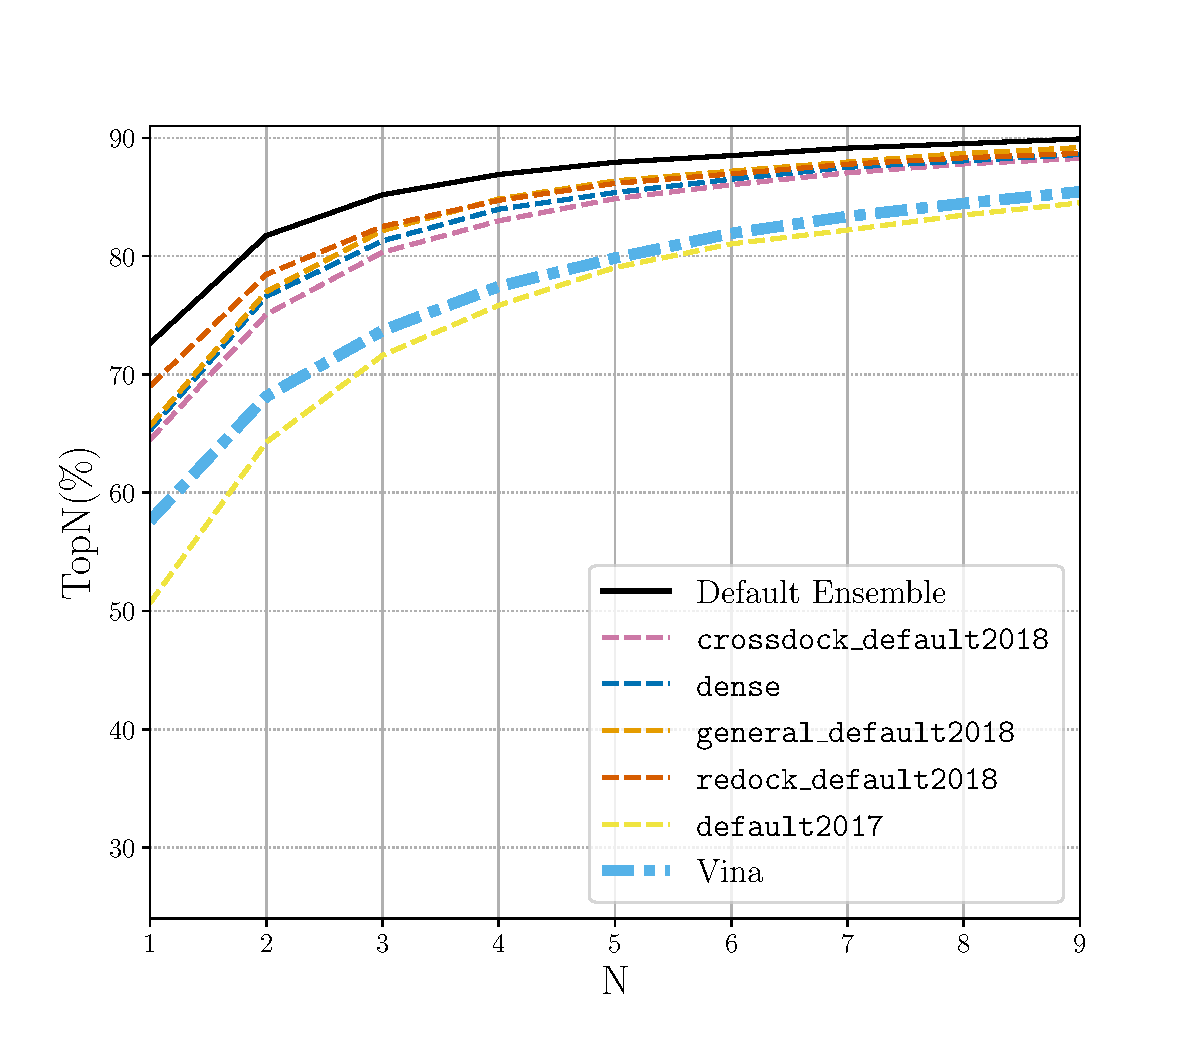
\includegraphics[width=\textwidth]{figures/redocking/rescore_single_models_line.pdf}
		\caption{Redocking}
		\label{fig:RescoreSingleRedock}
        \end{subfigure}    
	\begin{subfigure}[b]{0.48\textwidth}    
		\centering
		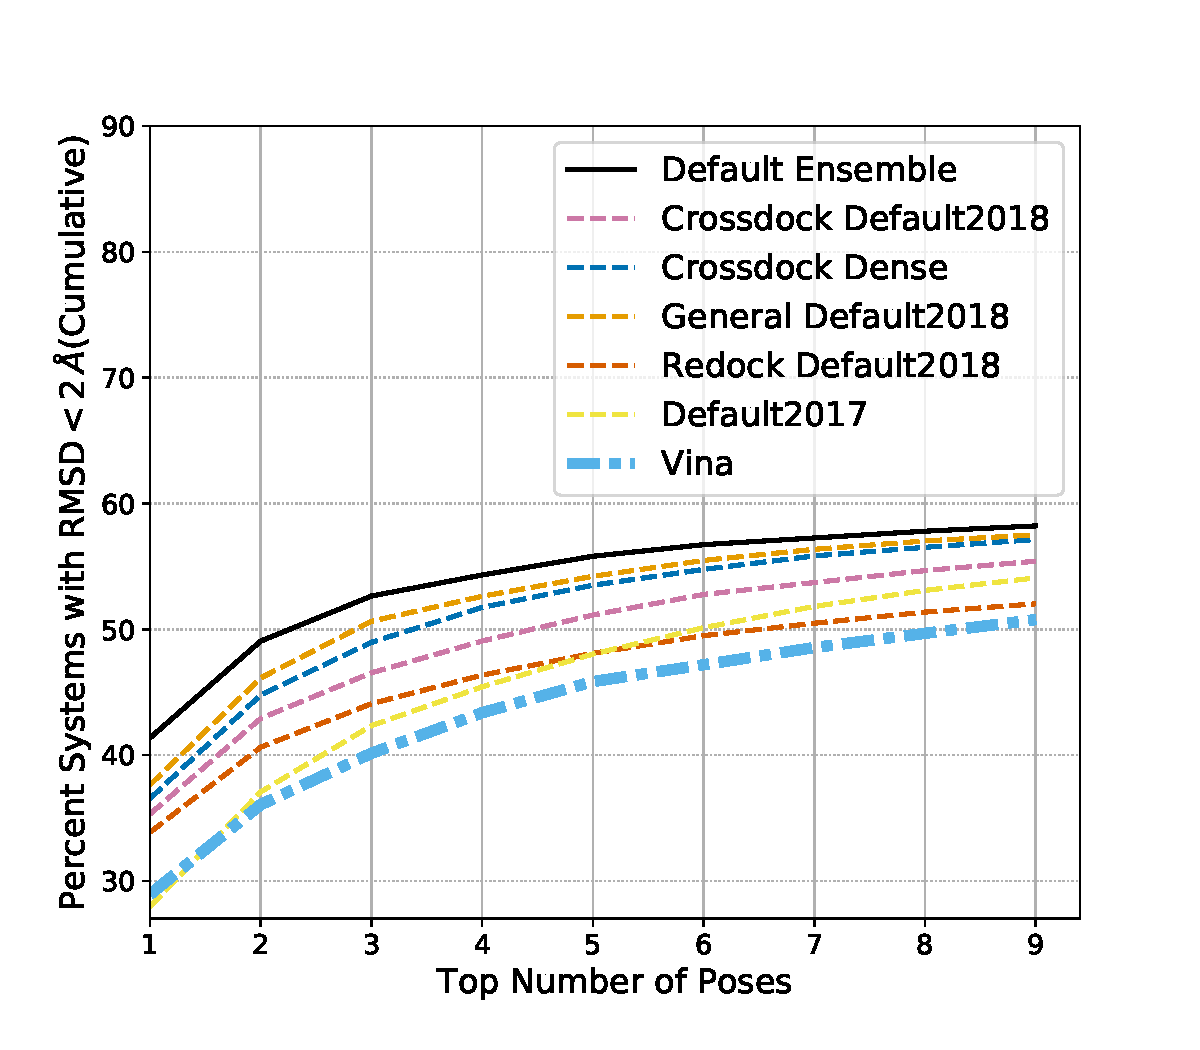
\includegraphics[width=\textwidth]{figures/crossdocking/rescore_single_models_line.pdf}
		\caption{Crossdocking}
		\label{fig:RescoreSingleCrossdock}
        \end{subfigure}    
	\caption{Docking using the single CNN models and the newly selected Default Ensemble for rescoring the output poses. The binding pocket is defined by the known binding pose.}
	\label{fig:RescoreSingle}
\end{figure}    
The iterative process for construction the default CNN ensemble, denoted Default Ensemble, is shown in Table \ref{tab:OptimalModelSelection}. The selected five selected models are Dense\_4, General\_Default2018\_3, Dense\_3, Crossdock\_Default2018, and Redock\_Default2018\_2. The performance of the model ensemble is compared to the single model options in Figure \ref{fig:RescoreSingle}. While nearly all models are able to rank poses with low RMSD higher than Vina, we can see that the newly selected Default Ensemble significantly outperforms all of the single models on both the redocking task and the crossdocking task.  

When the Default Ensemble is compared to the ensembles of each of the individual CNN model types, we see that the Default Ensemble is able to outperform all of the ensembles composed of one model type (Figure~\ref{fig:RescoreEnsemble}). The diversity of models within the Default Ensembles allows better ranking of the poses due to the diversity of training data and model architectures for each model type. The All Ensemble is the ensemble composed of all possible CNN models built-in to the \textsc{Gnina} software. The Default Ensemble is able to meet or exceed the performance of this large ensemble. The CNN models in the Default Ensemble are a subset of the 16 models in the All Ensemble. Reducing the number of models in the ensemble enables the computations to be several seconds faster for an average docking run (Figure~\ref{fig:OptimalRescore}). This reduction is likely due to the inclusion of only two of the Dense models which take the longest to run because of the high number of parameters in the model. The computational speedup afforded by the Default Ensemble over the All Ensemble increases when no GPU is used for docking (Figure: ~\ref{tab:OptimalRescoreNoGPU}). The computational speed boost can have a significant impact when performing a large number of docking runs or when there is no GPU available for enhanced parallelism of the scoring computation. The model ensemble selection procedure selected five CNN models whose combined performance on ranking low RMSD poses first beats the performance of the ensemble utilizing all of the built-in models while significantly reducing computational cost.

\begin{figure}
	\begin{subfigure}[b]{0.48\textwidth}
		\centering
		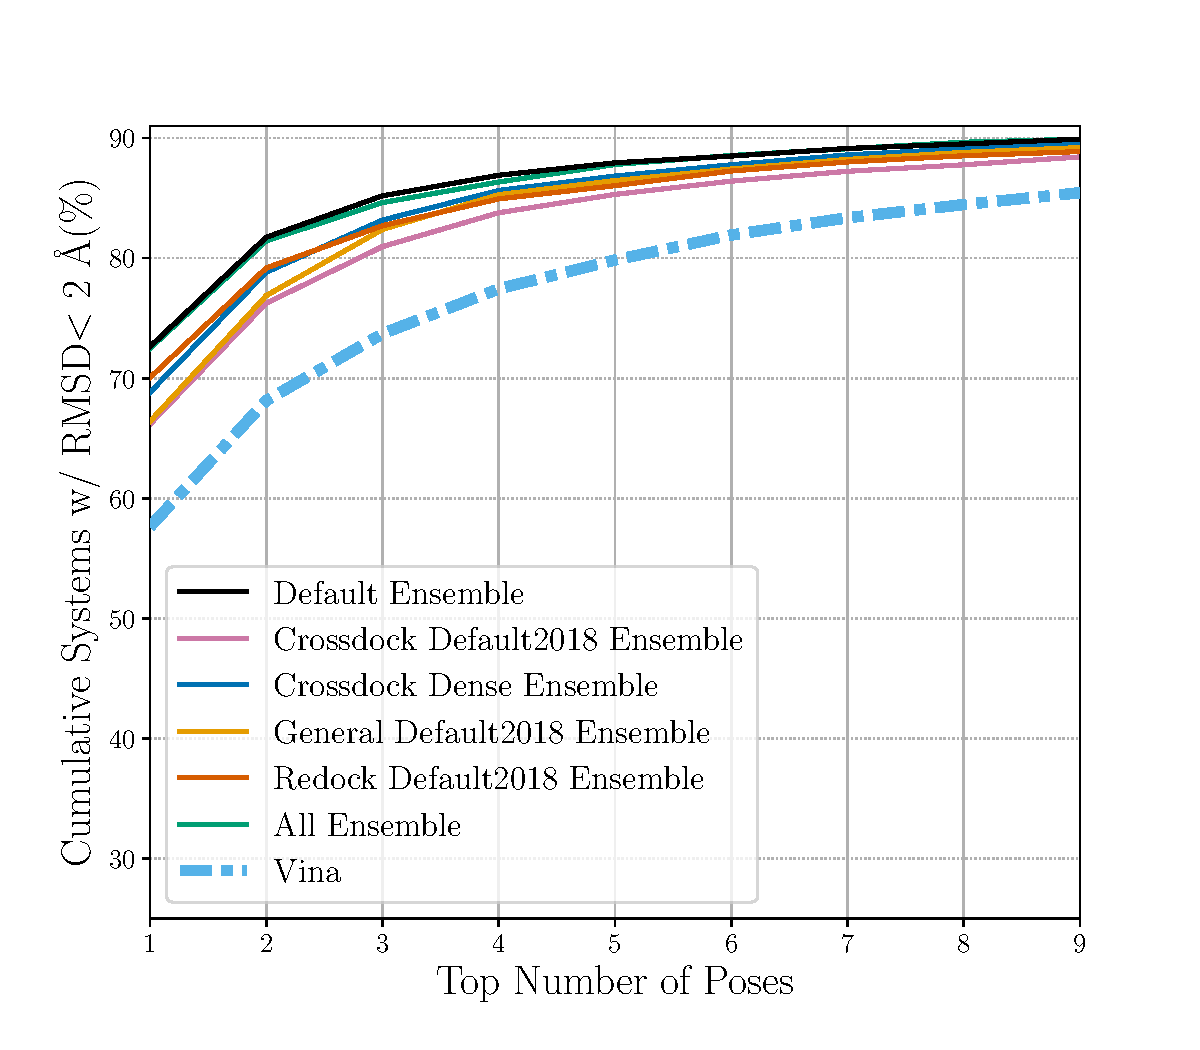
\includegraphics[width=\textwidth]{figures/redocking/rescore_ensembles_line.pdf}
		\caption{Redocking}
		\label{fig:RescoreEnsembleRedock}
        \end{subfigure}    
	\begin{subfigure}[b]{0.48\textwidth} 
		\centering
		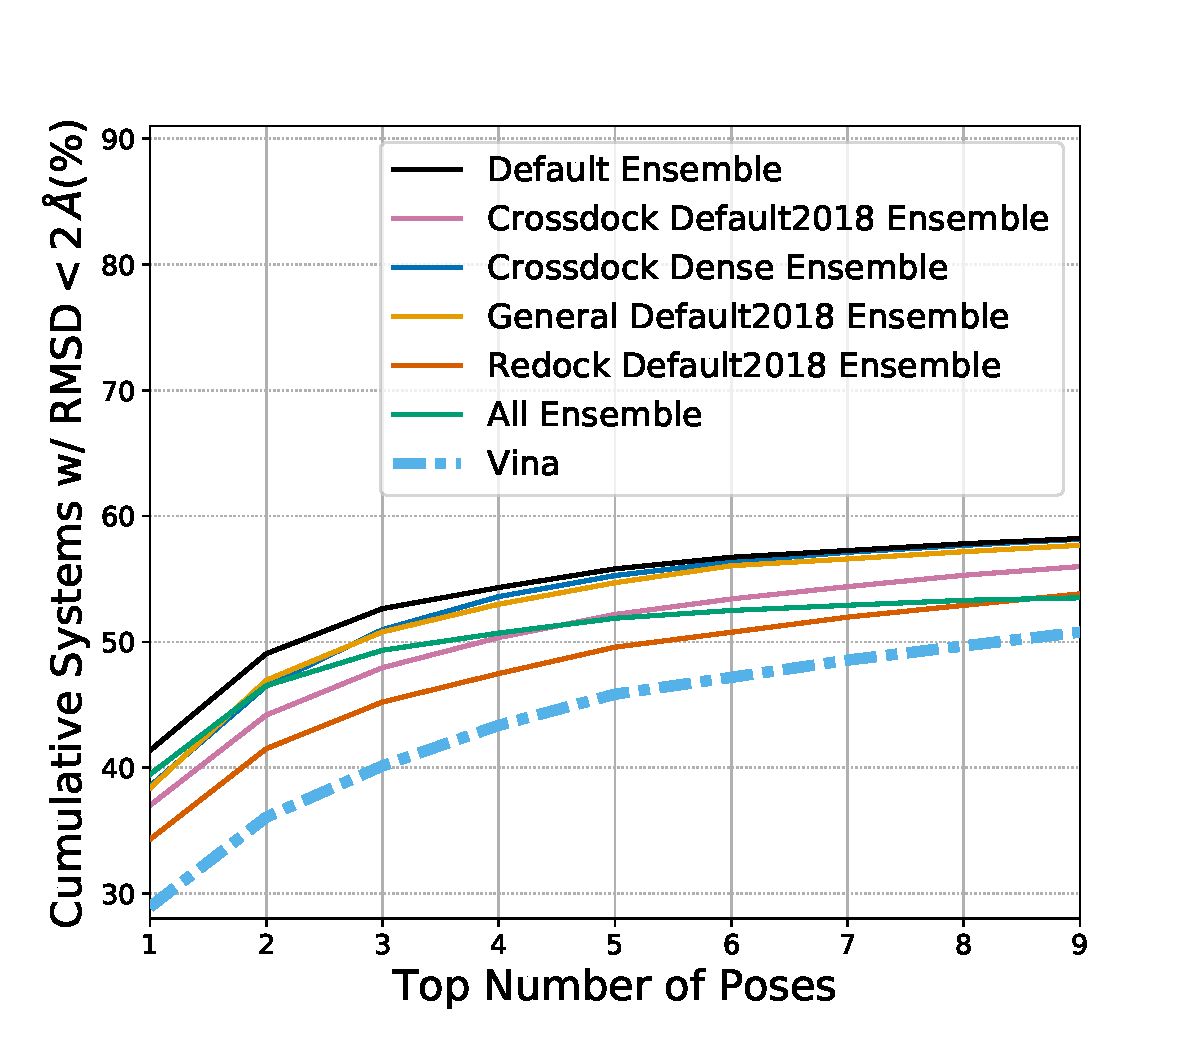
\includegraphics[width=\textwidth]{figures/crossdocking/rescore_ensembles_line.pdf}
		\caption{Crossdocking}
		\label{fig:RescoreEnsembleCrossdock}
        \end{subfigure}    
	\caption{Docking using the ensemble of each type of CNN model, the full ensemble of CNN models, and the newly selected Default Ensemble for rescoring the output poses. The binding pocket is defined by the known binding pose.}
	\label{fig:RescoreEnsemble}
\end{figure}    


\begin{figure}    
        \begin{subfigure}[b]{0.48\textwidth}
                \centering
                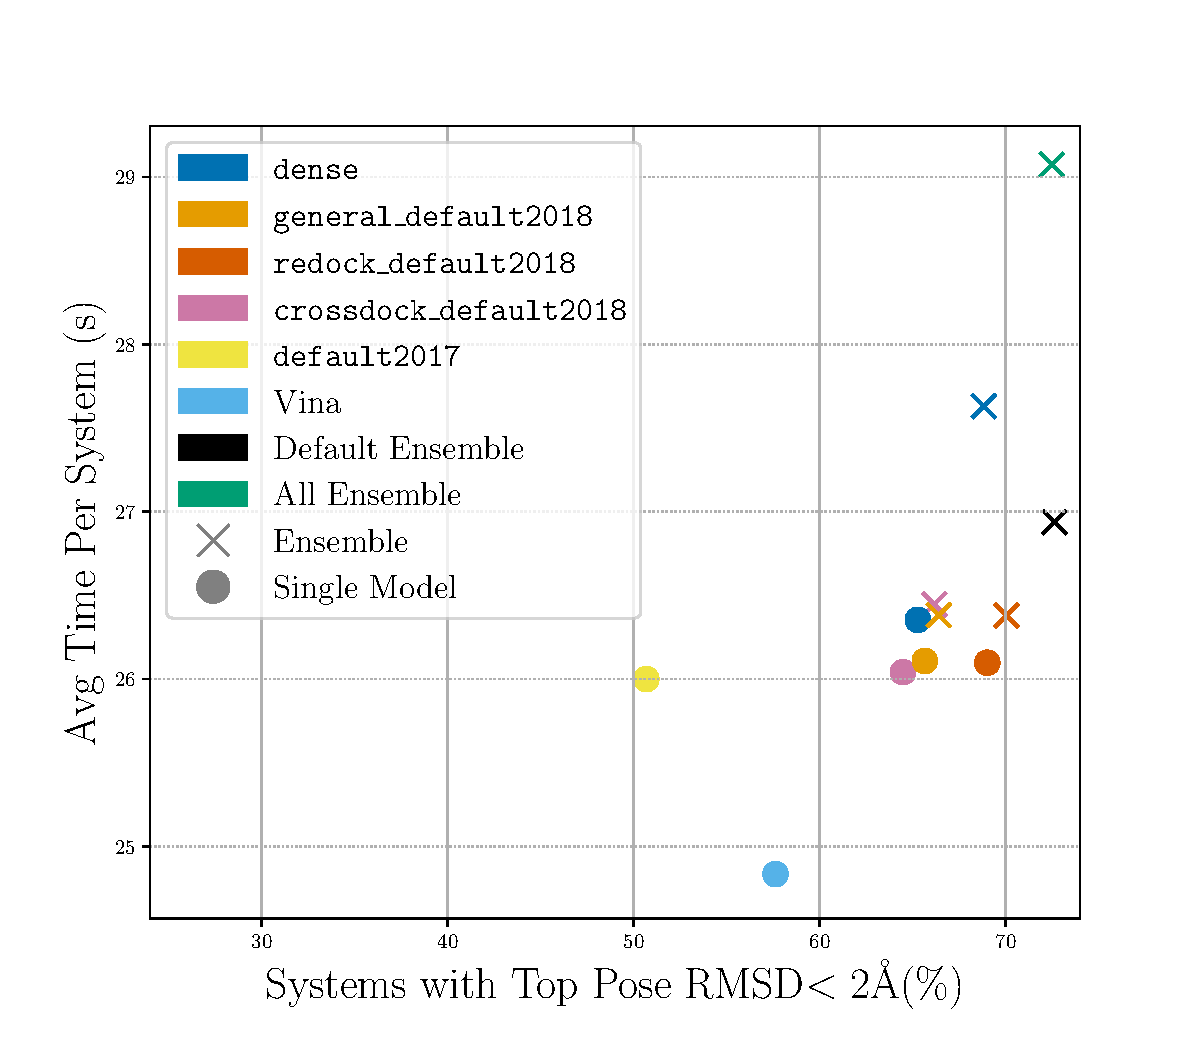
\includegraphics[width=\textwidth]{figures/redocking/gpu_models_line_rescore.pdf}
                \caption{Redocking}
                \label{fig:OptimalRescRD}
        \end{subfigure}    
        \begin{subfigure}[b]{0.48\textwidth}
                \centering
                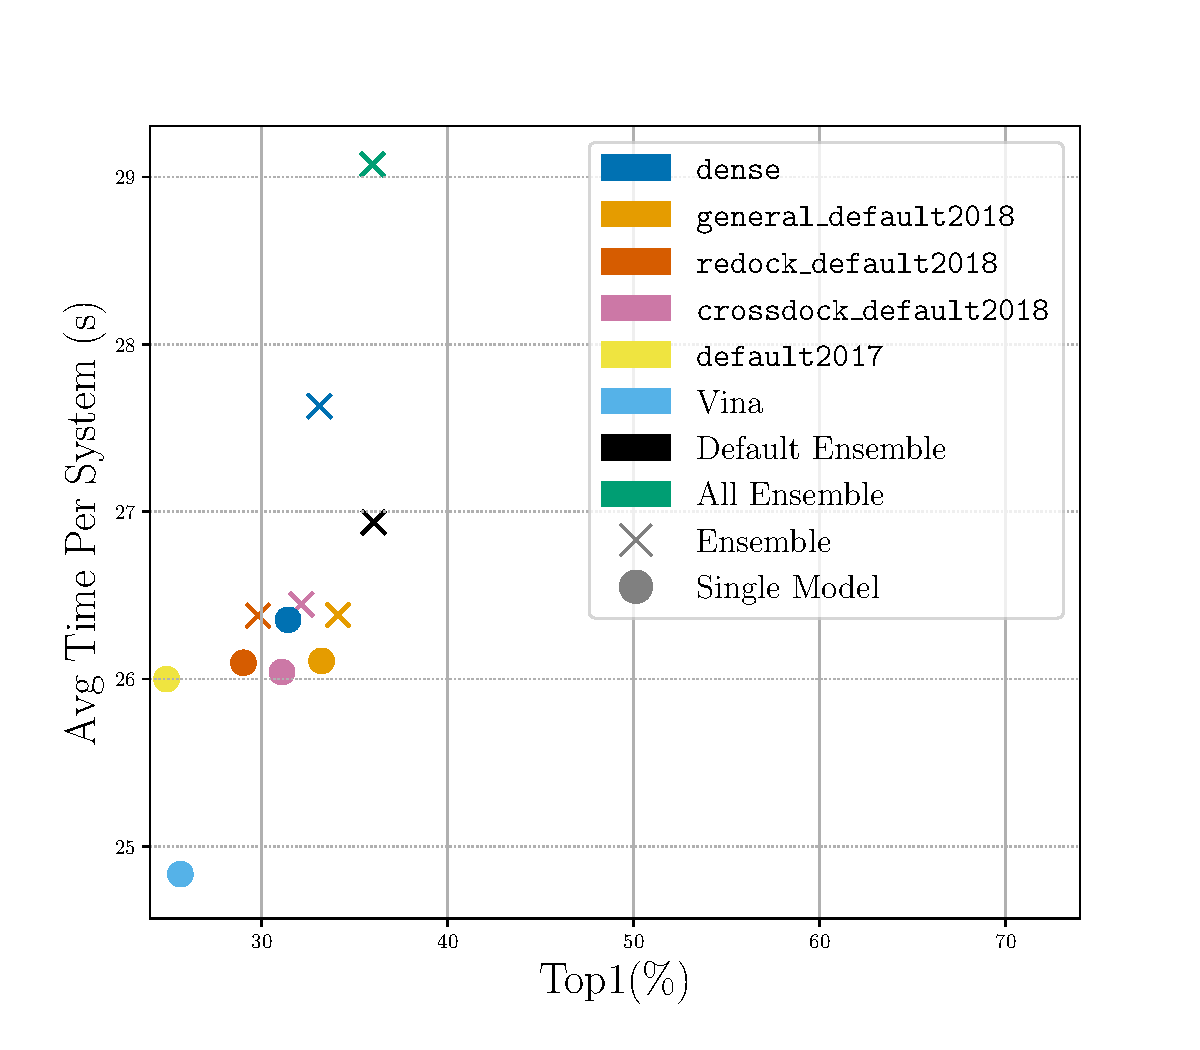
\includegraphics[width=\textwidth]{figures/crossdocking/gpu_models_line_rescore.pdf}
                \caption{Crossdocking}
                \label{fig:OptimalRescCD}
        \end{subfigure}    
        \caption{Evaluation of the average time to dock one protein-ligand system from the PDBbind core set v.2016. Computations performed on 1 RTX 2080Ti and 4 CPUs. }
        \label{fig:OptimalRescore}
\end{figure}    

\subsection{Default CNN Scoring Method}
 We evaluate the performance of the Default Ensemble with the ``rescore,'' ``refinement,'' and ``all'' options. However, the usage of the ``all'' option was unable to complete on the PDBbind Core set in a reasonable amount of time, so it was taken out of consideration. We are then left with comparing the ``refinement'' and ``rescoring'' options of the CNN scoring. We can see from Figure \ref{fig:CompareRescoreRefine} that the Default Ensemble performs nearly equally with either option. We can also see that using \texttt{cnn\_emp\_weight}, with both \texttt{mix\_emp\_energy} and \texttt{mix\_emp\_force}, does not significantly alter the docking performance when using the ``refinement'' option (Figure~\ref{fig:CNNEmpWeight}).

\begin{figure}    
        \begin{subfigure}[b]{0.48\textwidth}    
		\centering
		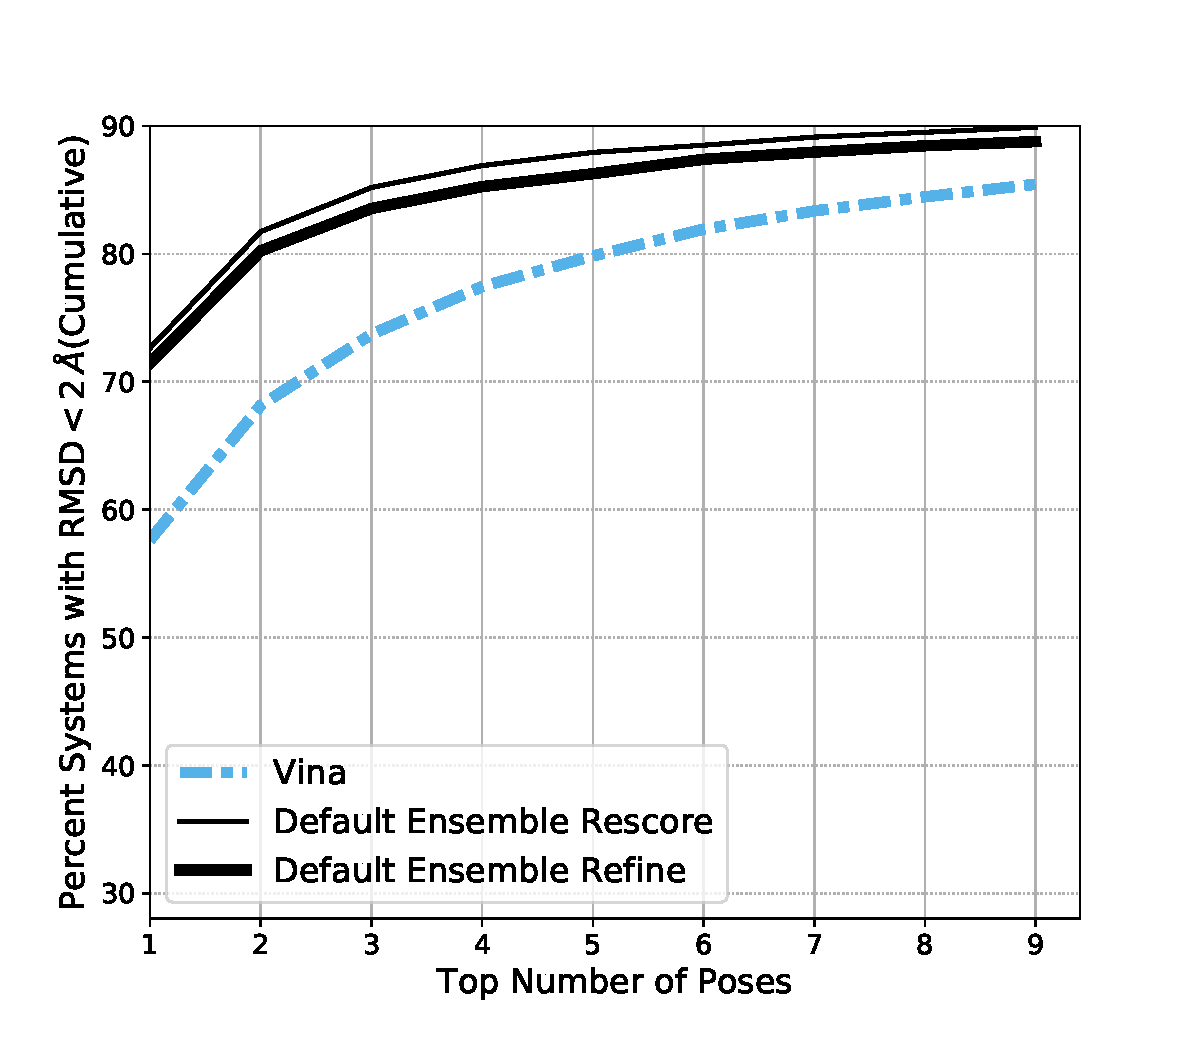
\includegraphics[width=\textwidth]{figures/redocking/rescore_vs_refine_line.pdf} 
		\caption{Redocking}
		\label{fig:CompareRescoreRefineRedock}
        \end{subfigure}    
        \begin{subfigure}[b]{0.48\textwidth}    
		\centering
		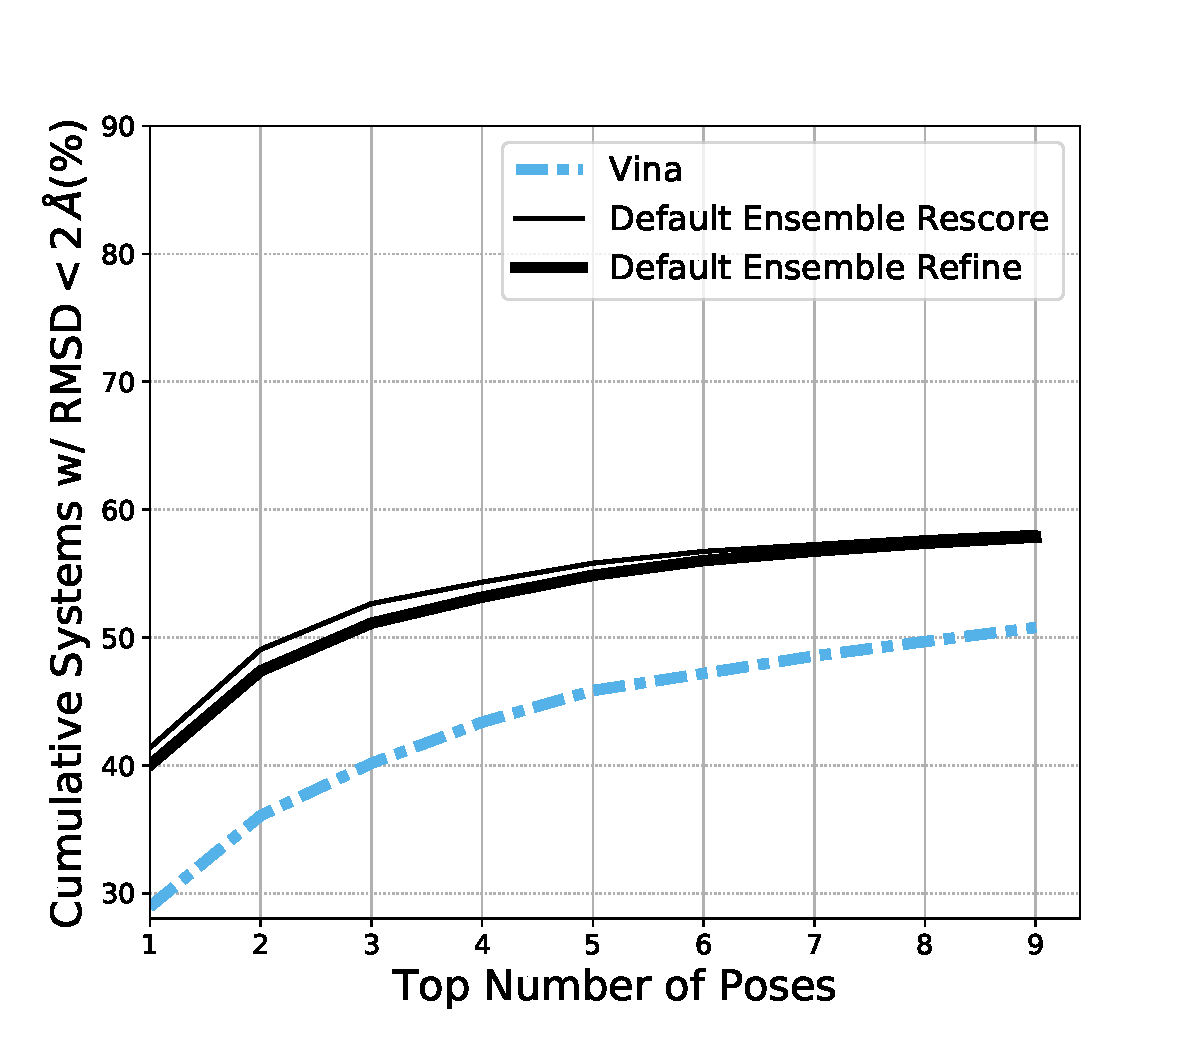
\includegraphics[width=\textwidth]{figures/crossdocking/rescore_vs_refine_line.pdf} 
		\caption{Crossdocking}
		\label{fig:CompareRescoreRefineCrossdock}
        \end{subfigure}    
	\caption{Comparing the Default CNN Ensemble for use in only rescoring of the poses output by the Monte Carlo chains or the refinement of the poses followed by a rescoring of the poses}
	\label{fig:CompareRescoreRefine}
\end{figure}    

However, from looking at the average time to perform molecular docking for one system we see that ``refinement'' takes an order of magnitude longer than ``rescoring'' (Figure~\ref{fig:RefineTiming}). Time for performing the ``rescoring'' on an average system is similar to the time to perform docking with the Vina scoring function for an average protein-ligand system in the core set. Therefore, we select ``rescore'' as the default option for the CNN scoring due to its performance and timing.

\subsection{Settings Exploration}

First we evaluate the size of the targetted binding site (box). The \texttt{autobox\_add} parameter increases the search space for the docking program to be larger than the rectangular prism defined by the autobox ligand input to \textsc{Gnina}. In both redocking and crossdocking (Figure \ref{fig:AutoboxAdd}), the expansion of the search space decreases performance as the expanded search space makes the sampling problem more difficult. A higher value of \texttt{autobox\_add} aids the docking procedure in finding the correct binding site when the binding site is incorrectly identified, while a low value artificially improves docking performance when the binding pose is known. We therefore select a default value of 4 for \texttt{autobox\_add} to keep the box small while still providing room for error in the selection of the binding site.

\begin{figure}    
        \begin{subfigure}[b]{0.48\textwidth}    
		\centering
		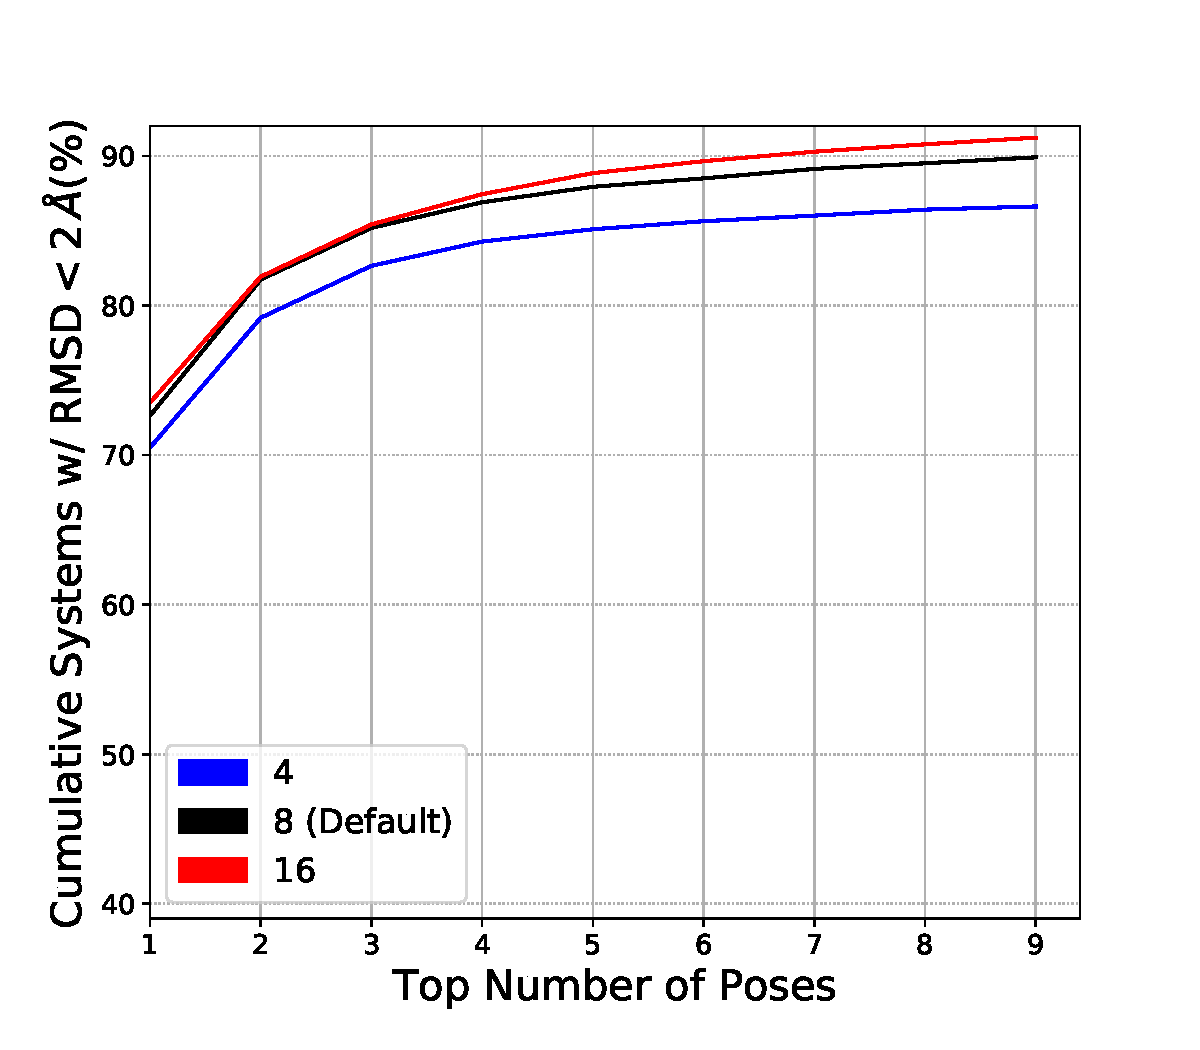
\includegraphics[width=\textwidth]{figures/redocking/sweep_exhaustiveness_line.pdf}
		\caption{Redocking}
		\label{fig:exhaustiveness rd}
        \end{subfigure}    
        \begin{subfigure}[b]{0.48\textwidth}    
		\centering
		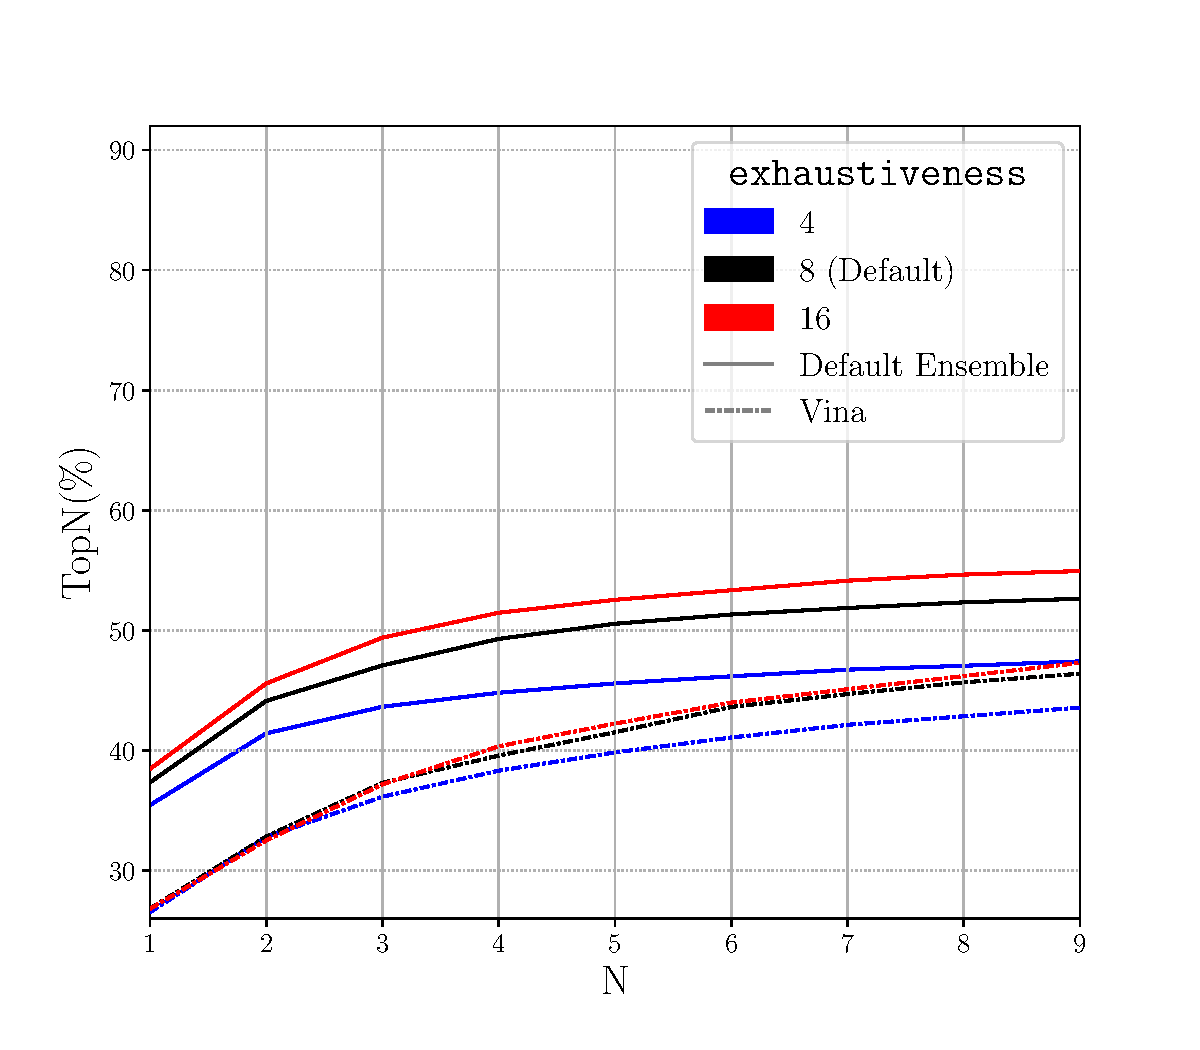
\includegraphics[width=\textwidth]{figures/crossdocking/sweep_exhaustiveness_line.pdf}
		\caption{Crossdocking}
		\label{fig:exhaustiveness cd}
        \end{subfigure}    
	\caption{Evaluating the role of exhaustiveness in the performance of docking with the Default CNN Ensemble}
	\label{fig:exhaustiveness}
\end{figure}    

Changes in the exhaustiveness alter the amount of sampling that occurs. When the exhaustiveness is increased, we see an increase in the performance of docking. This is as expected as more Monte Carlo chains randomly mutating the ligand conformation provides the docking procedure with more opportunities to randomly sample the correct answer. However, this increase in performance seems to reach limited gains after a value of 8. An exhaustiveness of 16 provides some performance boost, but this boost may be accompanied by a doubling of the computational time. The Monte Carlo chains are evaluated in parallel, but parallelism is limited by the number of cores available to \textsc{Gnina}. So if the exhaustiveness is greater than the CPUs provided to \textsc{Gnina}, the number of simultaneously running Monte Carlo chains is equal to the number of CPUs. Therefore, in typical usage of \textsc{Gnina}, an exhaustiveness level of 8 is sufficient for adequate performance levels while minimizing the computational load when targetting a specific binding site. 

Changes to the CNN rotations do not significantly change the scoring of the Default Ensemble (Figure \ref{fig:CNNRot}). The CNN Ensemble is able to determine the correct score for the ligand pose regardless of the rotation of the ligand and protein complex. Altering the value of the minimum RMSD filter does not change the results of the docking (Figure \ref{fig:RMSDFilter}).  Filtering out poses with similar conformations increases the diversity of poses that the CNN ensemble ranks. However, the CNN ensemble is able to accurately rank the poses it sees, providing high scores to poses with low RMSD to the known binding pose.

\begin{figure}    
        \begin{subfigure}[b]{0.48\textwidth}    
		\centering
		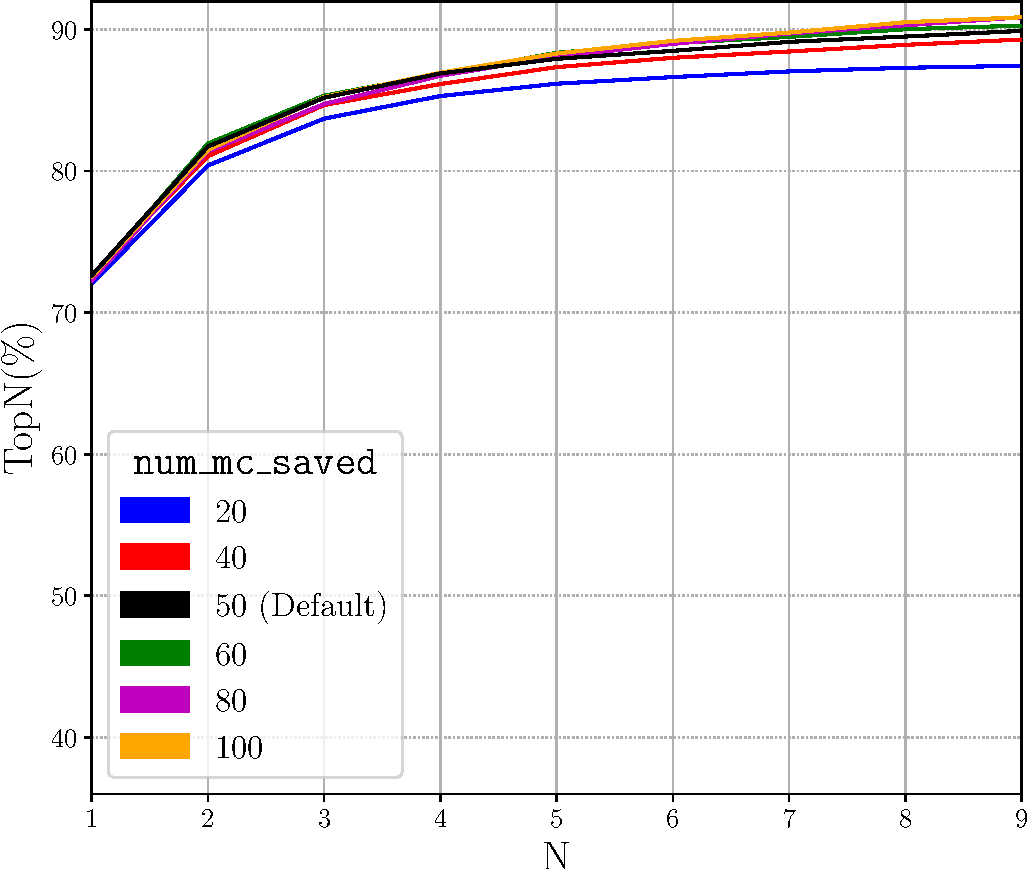
\includegraphics[width=\textwidth]{figures/redocking/sweep_mcsaved_line.pdf}
		\caption{Redocking}
		\label{fig:mcsaved rd}
        \end{subfigure}    
        \begin{subfigure}[b]{0.48\textwidth}    
		\centering
		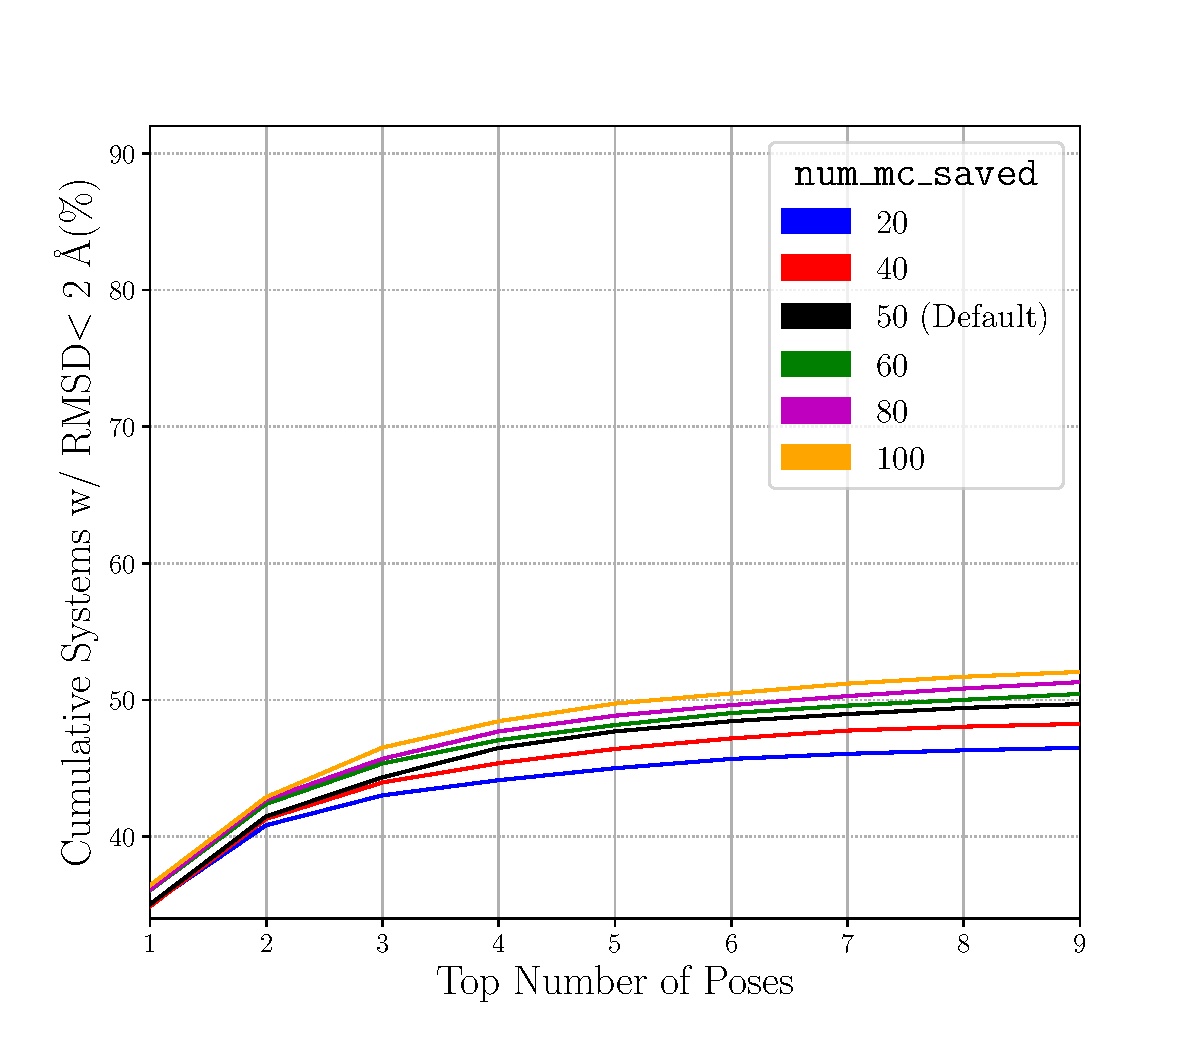
\includegraphics[width=\textwidth]{figures/crossdocking/sweep_mcsaved_line.pdf}
		\caption{Crossdocking}
		\label{fig:mcsaved cd}
        \end{subfigure}    
	\caption{Evaluation of the Number of Monte Carlo Saved in the performance of docking with the Default CNN Ensemble}
	\label{fig:mcsaved}
\end{figure}    

Increasing the \texttt{num\_mc\_saved} parameter increases the chances of sampling accurate docking poses. Since the molecular docking procedure is a sampling problem, with increased output conformations from each Monte Carlo chain there is an increased likelihood of finding the correct answer. However, this will also increase computational time, due to more poses requiring refinement and final scoring by the CNN model(s). As the number of Monte Carlo saved gets closer to 100, we see that the docking performance boost is reduced. Therefore, we select a value of 50 for the number of Monte Carlo saved to minimize the computational overhead while still increasing the performance of the docking routine. The \texttt{num\_mc\_saved} and \texttt{num\_modes} affect one another; the number of poses saved from each Monte Carlo chain is the maximum of the two values. When looking at the first 9 poses, we see a marked increase in the performance of docking with a substantially greater value for the number of output poses (\texttt{num\_modes}). This is due to \texttt{num\_modes} forcing each Monte Carlo chain to output a number of poses greater than \texttt{num\_mc\_saved}. Increasing the default value of \texttt{num\_modes} will again increase computational overhead, so the default value is set to 9. 

\begin{figure}    
        \begin{subfigure}[b]{0.48\textwidth}    
		\centering
		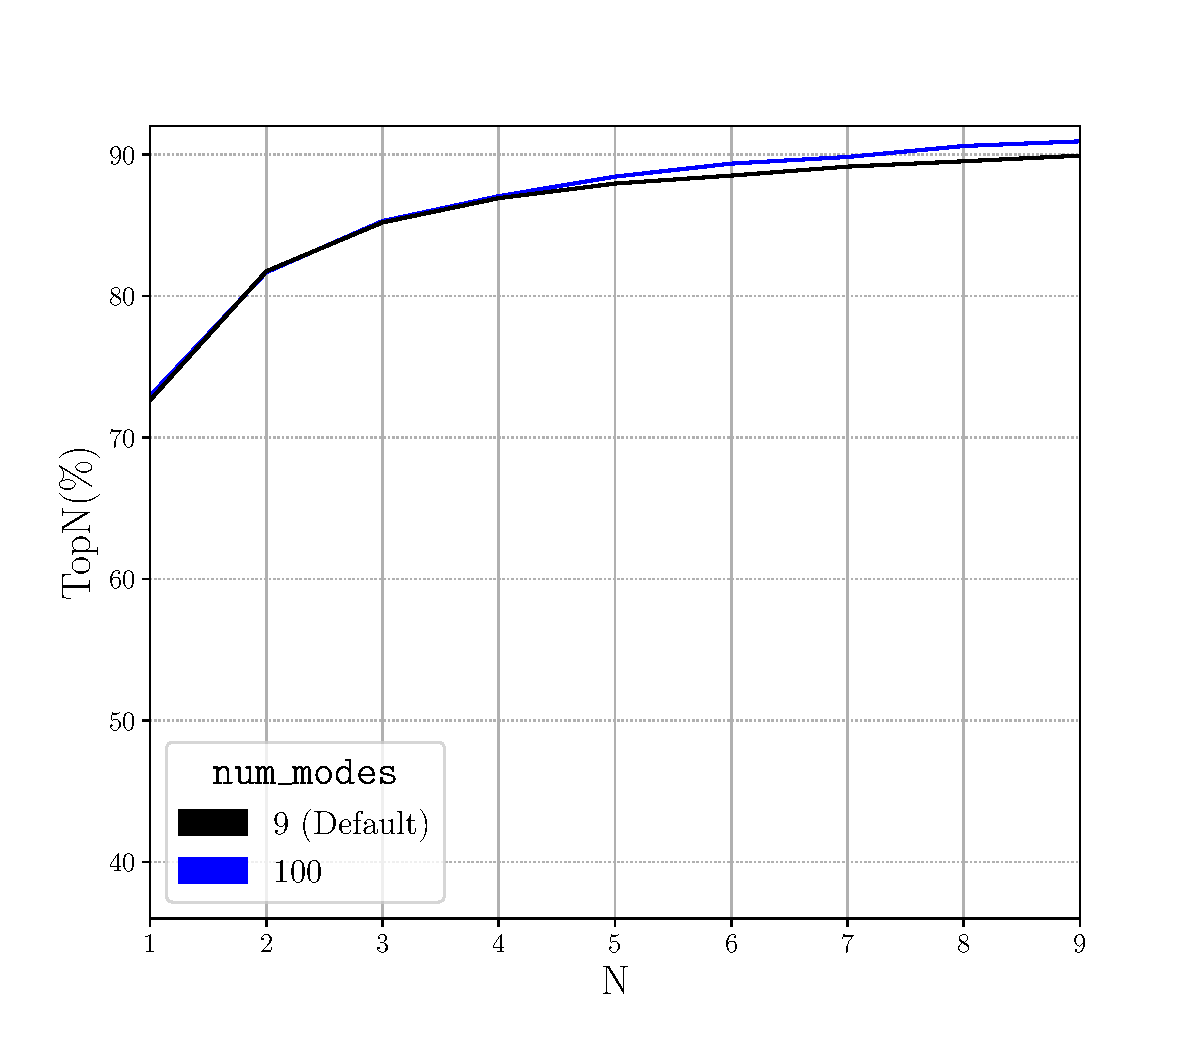
\includegraphics[width=\textwidth]{figures/redocking/sweep_num_modes_line.pdf}
		\caption{Redocking}
		\label{fig:num modes rd}
        \end{subfigure}    
        \begin{subfigure}[b]{0.48\textwidth}    
		\centering
		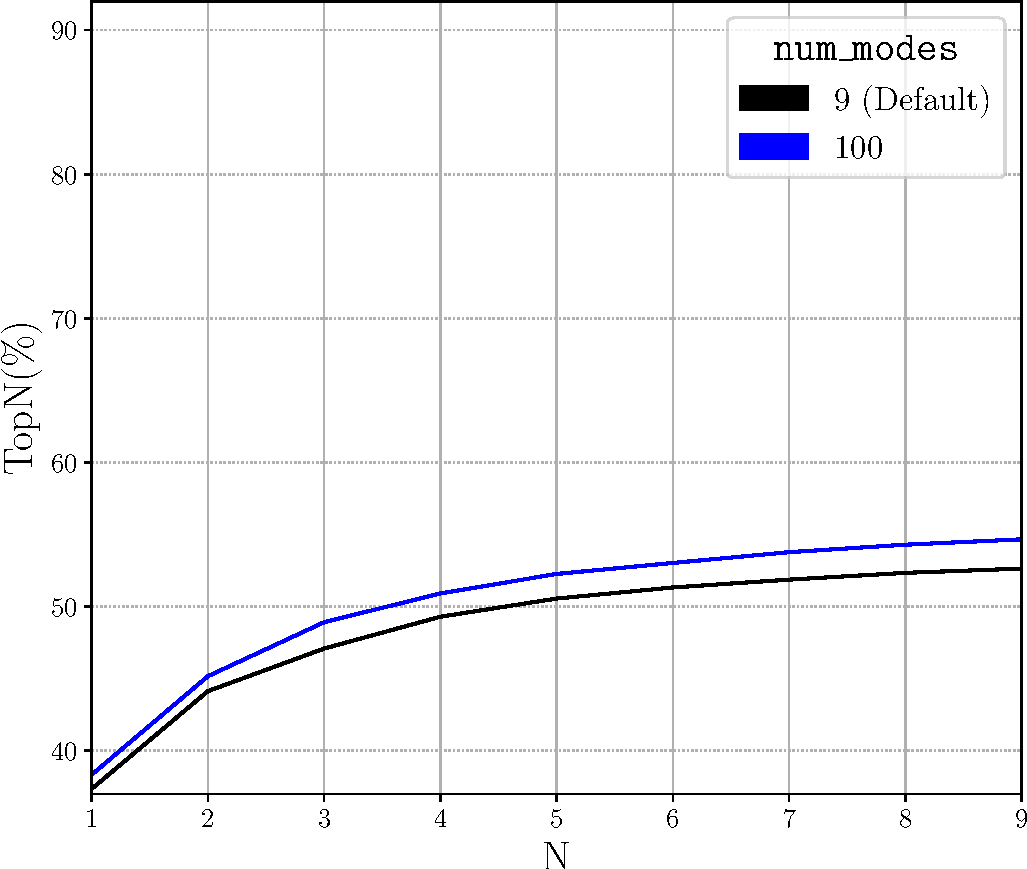
\includegraphics[width=\textwidth]{figures/crossdocking/sweep_num_modes_line.pdf}
		\caption{Crossdocking}
		\label{fig:num modes cd}
        \end{subfigure}    
	\caption{Evaluating a much greater number of modes on the performance of docking with the Default CNN Ensemble}
	\label{fig:num modes}
\end{figure}

\subsection{Whole Protein Docking}

Finally, we evaluate the performance of docking when using the whole protein as the defined `binding site.' The performance of docking is expected to be reduced as the sampling space has been significantly increased. When using the whole protein for the sampling space, the sampling procedure tends to get stuck at locations distant from the actual binding site. It is difficult to move away from high scoring locations due to high energy boundaries. Figure~\ref{fig:WholeProteinExh} shows the performance of both Vina and the Default CNN Ensemble are reduced from when the binding pocket was explicitly defined. With whole protein docking we see greater increases in performance with increased sampling (\texttt{exhaustiveness}). This boost in performance is larger than when the binding pocket is defined explicitly and, as shown in Figure~\ref{fig:WholeProteinExh}, does not exhibit the same diminishing returns. For this reason, when performing whole protein docking, we recommend setting the value of exhaustiveness as high as possible given the timing constraints of the problem at hand.

\begin{figure}    
        \begin{subfigure}[b]{0.48\textwidth}    
    		\centering
    		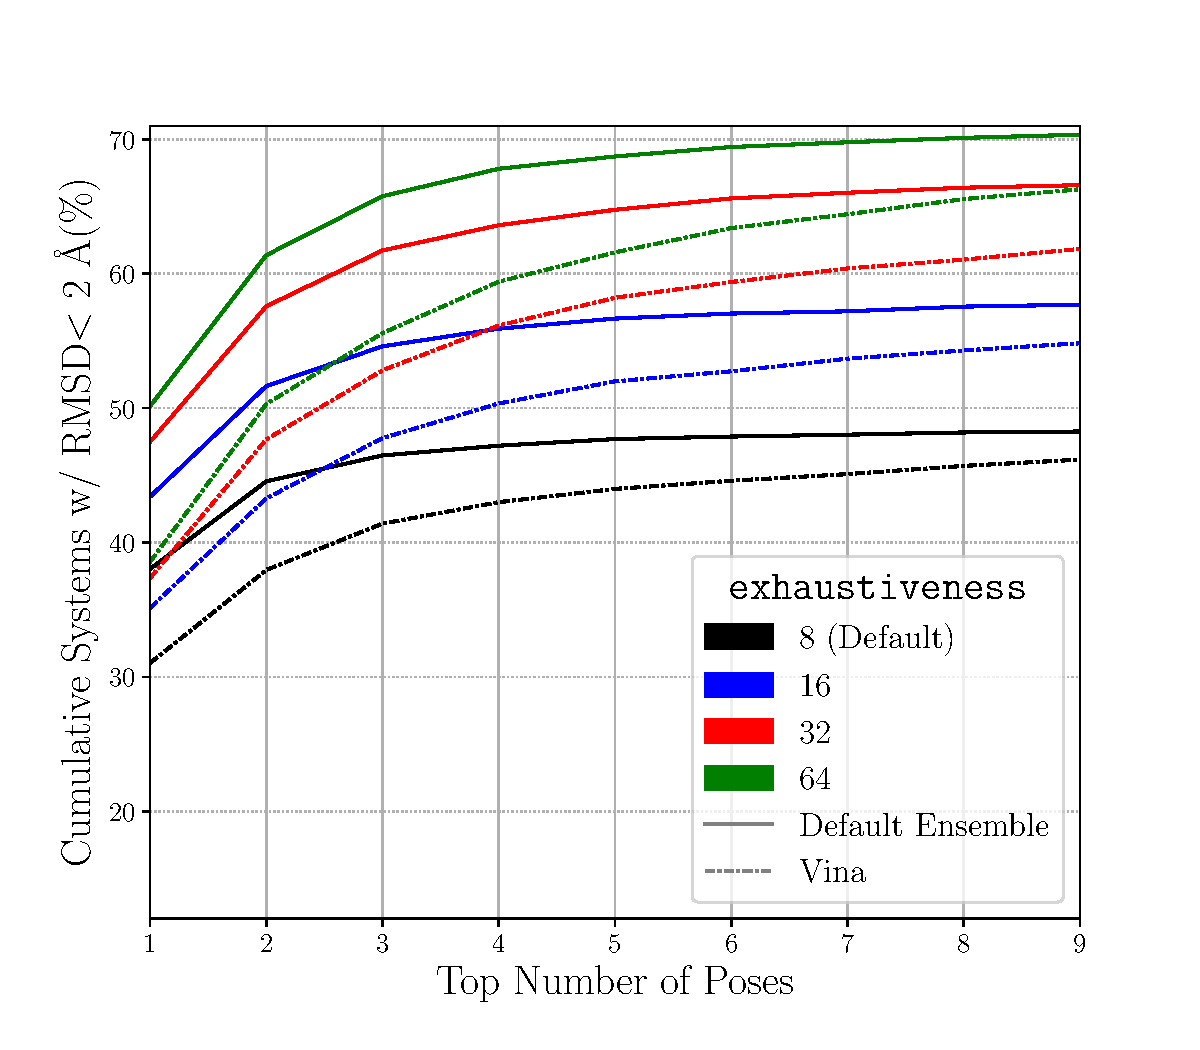
\includegraphics[width=\textwidth]{figures/redocking/whole_ptn_sweep_exhaustiveness_line.pdf}
    		\caption{Redocking}
            \label{fig:WholeProteinExhRD}
        \end{subfigure}    
        \begin{subfigure}[b]{0.48\textwidth}    
    		\centering
    		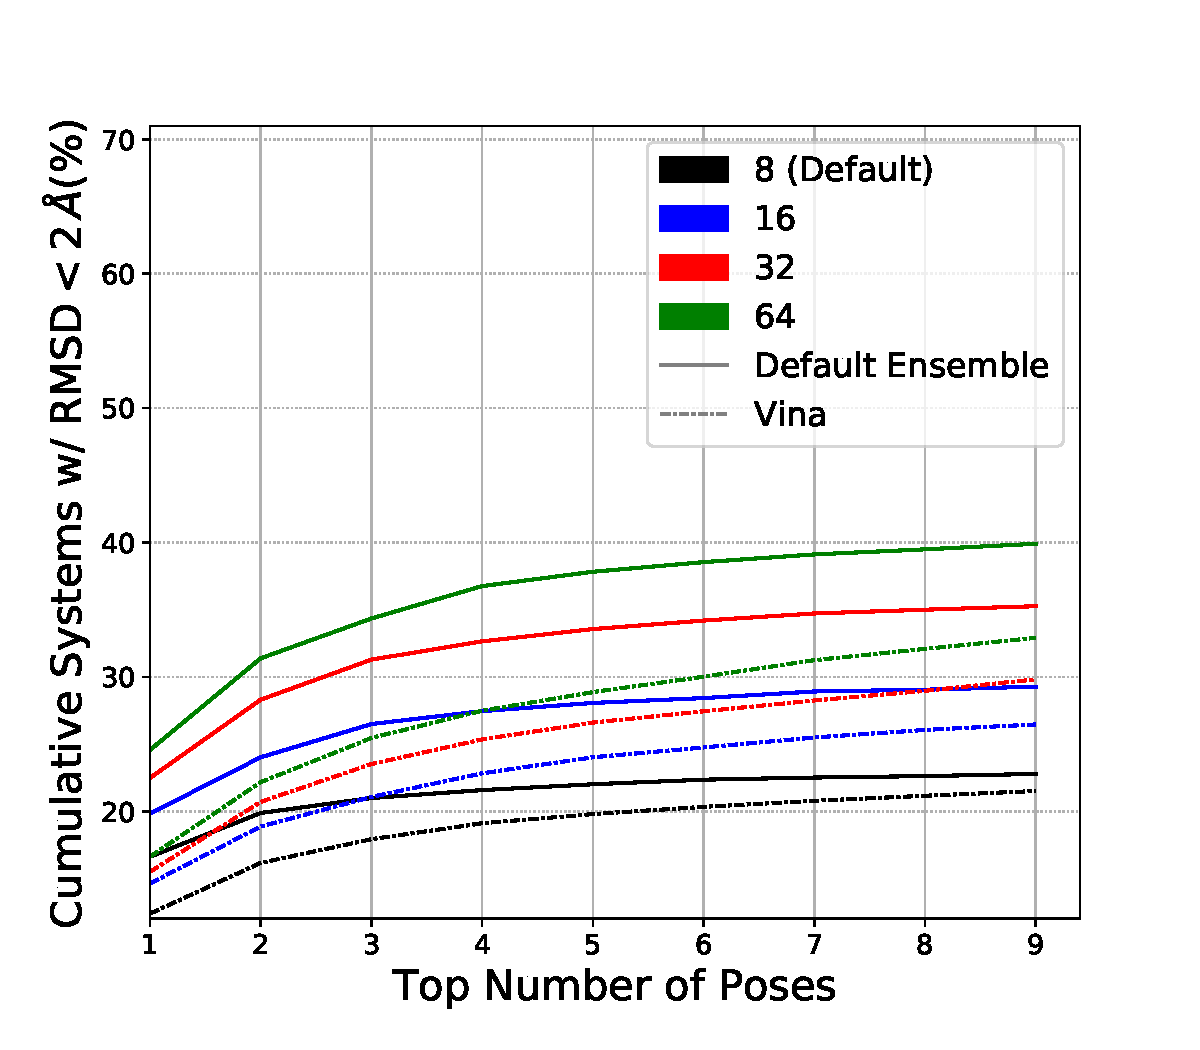
\includegraphics[width=\textwidth]{figures/crossdocking/whole_ptn_sweep_exhaustiveness_line.pdf}
    		\caption{Crossdocking}
            \label{fig:WholeProteinExhCD}
        \end{subfigure}    
	\caption{Increasing the exhaustiveness when using the whole protein as the binding box}
        \label{fig:WholeProteinExh}
\end{figure}

\subsection{CNN Scoring Performance}
We have evaluated all of the \textsc{Gnina} models on subsets of the data that were not seen by any of the CNN models during training to ensure that the CNN models are able to generalize to unseen protein-ligand systems. We also show the Vina results for the same subset of protein-ligand systems. First we evaluate on the systems within the PDBbind refined set v.2019 and not within the PDBbind general set v.2017. This removes all of the protein-ligand pairs in the training sets for the General\_Default2018 and Default2017 CNN models.
\begin{figure}    
	\begin{subfigure}[b]{0.48\textwidth}    
		\centering
		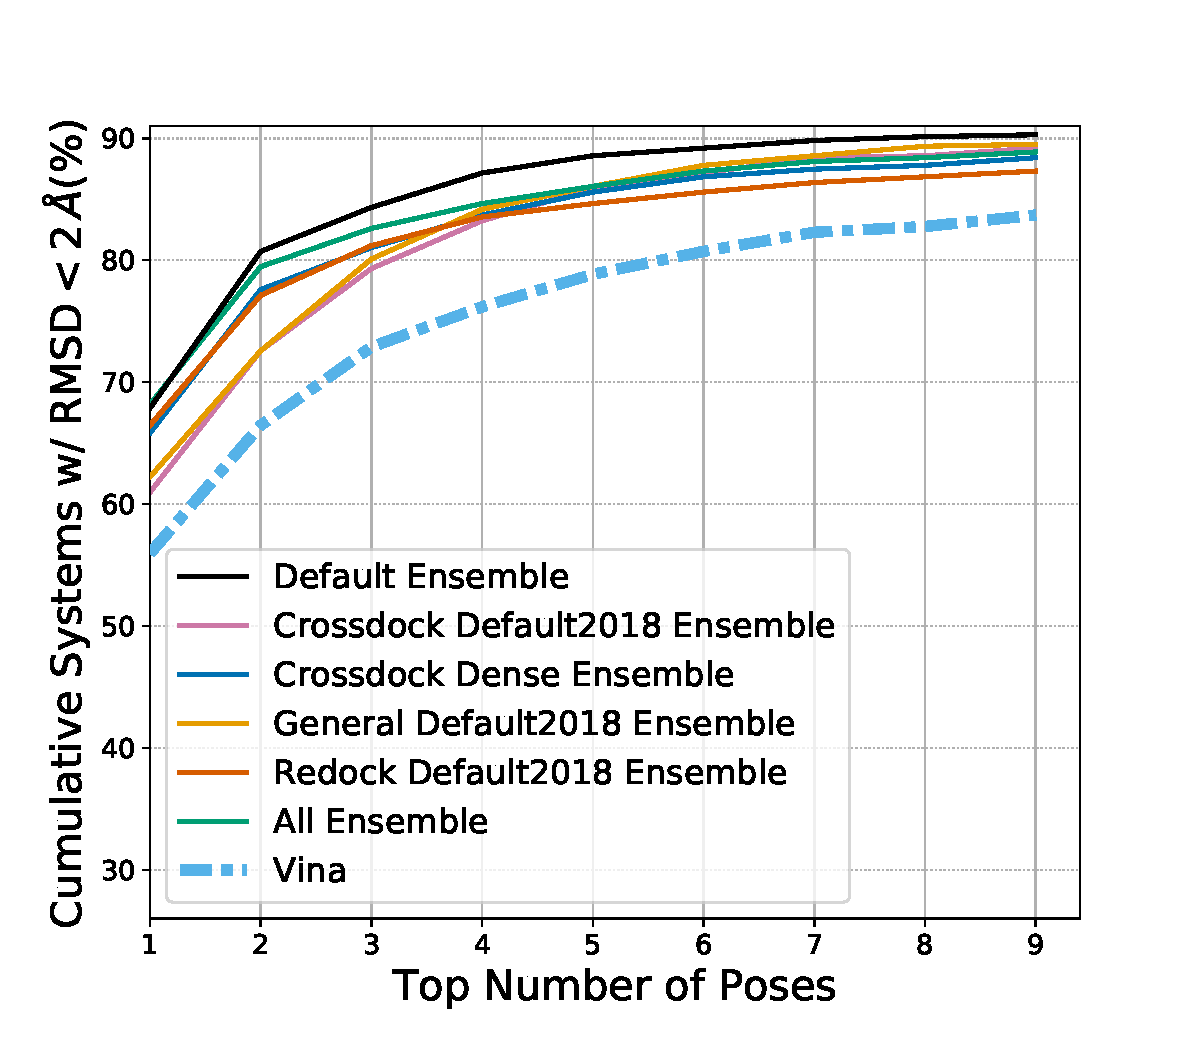
\includegraphics[width=\textwidth]{figures/redocking/ensemble_models_no2017_line.pdf}
		\caption{Redocking Ensembles}
		\label{fig:No2017NoCD20EnsRD}
    \end{subfigure}    
    \begin{subfigure}[b]{0.48\textwidth}    
		\centering
		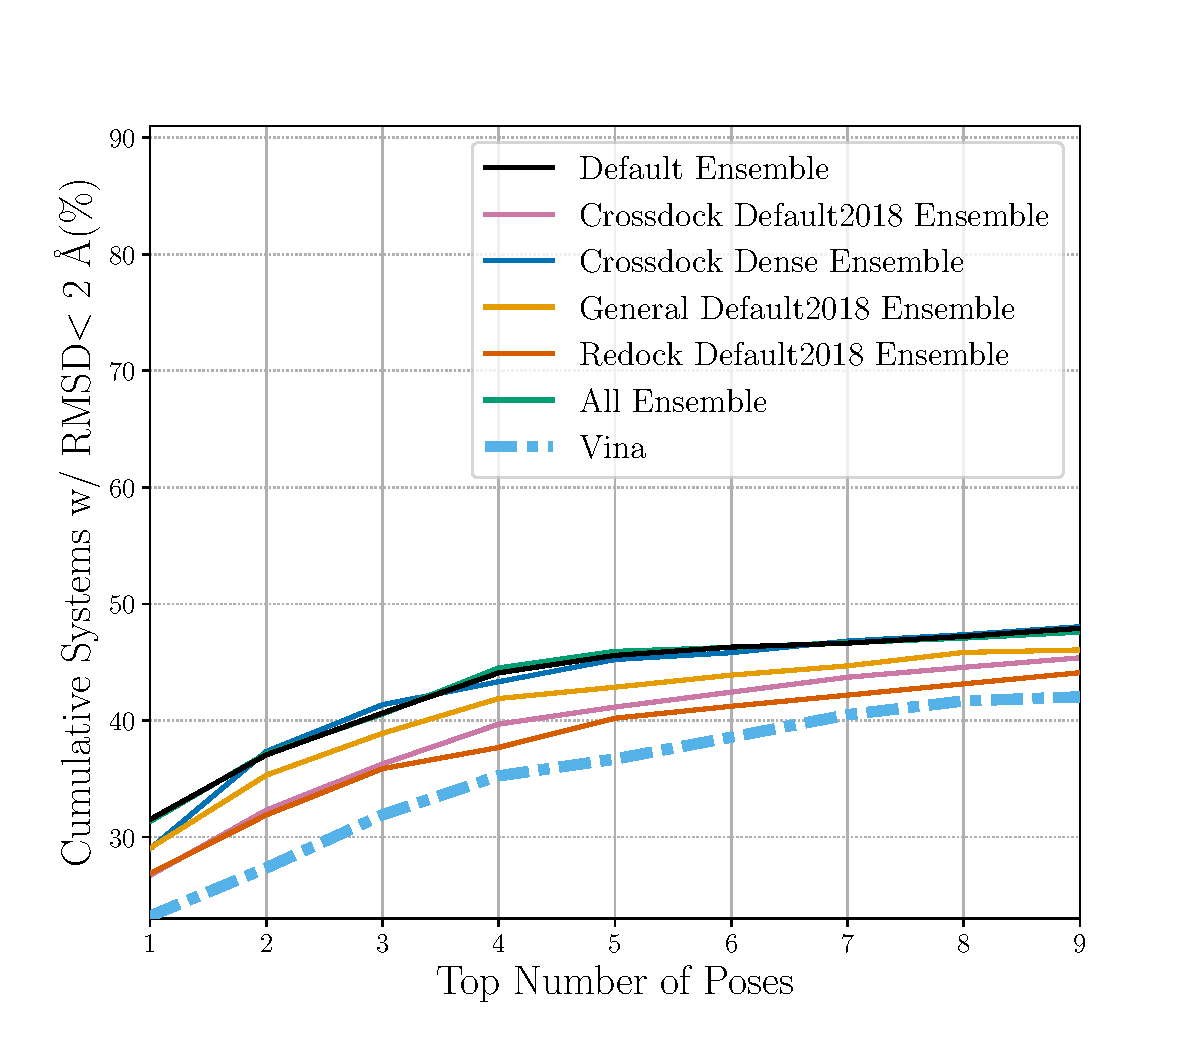
\includegraphics[width=\textwidth]{figures/crossdocking/ensemble_models_no2017_line.pdf}
		\caption{Crossdocking Ensembles}
                \label{fig:No2017NoCD20EnsCD}
    \end{subfigure}
	\caption{CNN model ensembles evaluated on the subset of systems not present in the PDBbind general set v.2017. Ensemble models used with the default arguments defined above.}
	\label{fig:No2017}
\end{figure}
The performance of each of the ensembles drops on this split of the data, but the models are still able to more accurately rank the poses than the Vina scoring function. The top pose performance for the Default Ensemble drops from 72\% to 67\% and 41\% to 39\% for redocking and crossdocking, respectively. While the top pose performance for Vina scoring drops from 58\% to 56\% and 29\% to 27\% for redocking and crossdocking, respectively. The top pose performance decrease of the General\_Default2018 Ensemble is similar to that of both the Default Ensemble and Vina scoring: 66\% to 62\% and 38\% to 36\% for redocking and crossdocking, respectively.

Next we evaluate on a split that removes any systems which were in either the PDBbind general set v.2017 or the Crossdock2020 dataset; this removes any of the proteins or ligands which were in the training sets of any of the CNN models. The CNN models docking performance decrease relative to the full sets when looking at the top pose, (Figure~\ref{fig:No2017NoCD20}). Redocking top pose performance drops from 72\% to 68\% on the Default Ensemble for the filtered set and the full set, respectively, while Vina remains at about 57\%. Crossdocking top pose performance increases from 41\% to 46\% for the Default Ensemble and decreases from 28\% to 26\% when using the Vina scoring function. Overall, the Default Ensemble still shows a strong docking performance boost when used to rescore poses rather than using the Vina scoring function to score poses even on protein-ligand systems not seen during training.

\begin{figure}    
        \begin{subfigure}[b]{0.48\textwidth}    
		\centering
		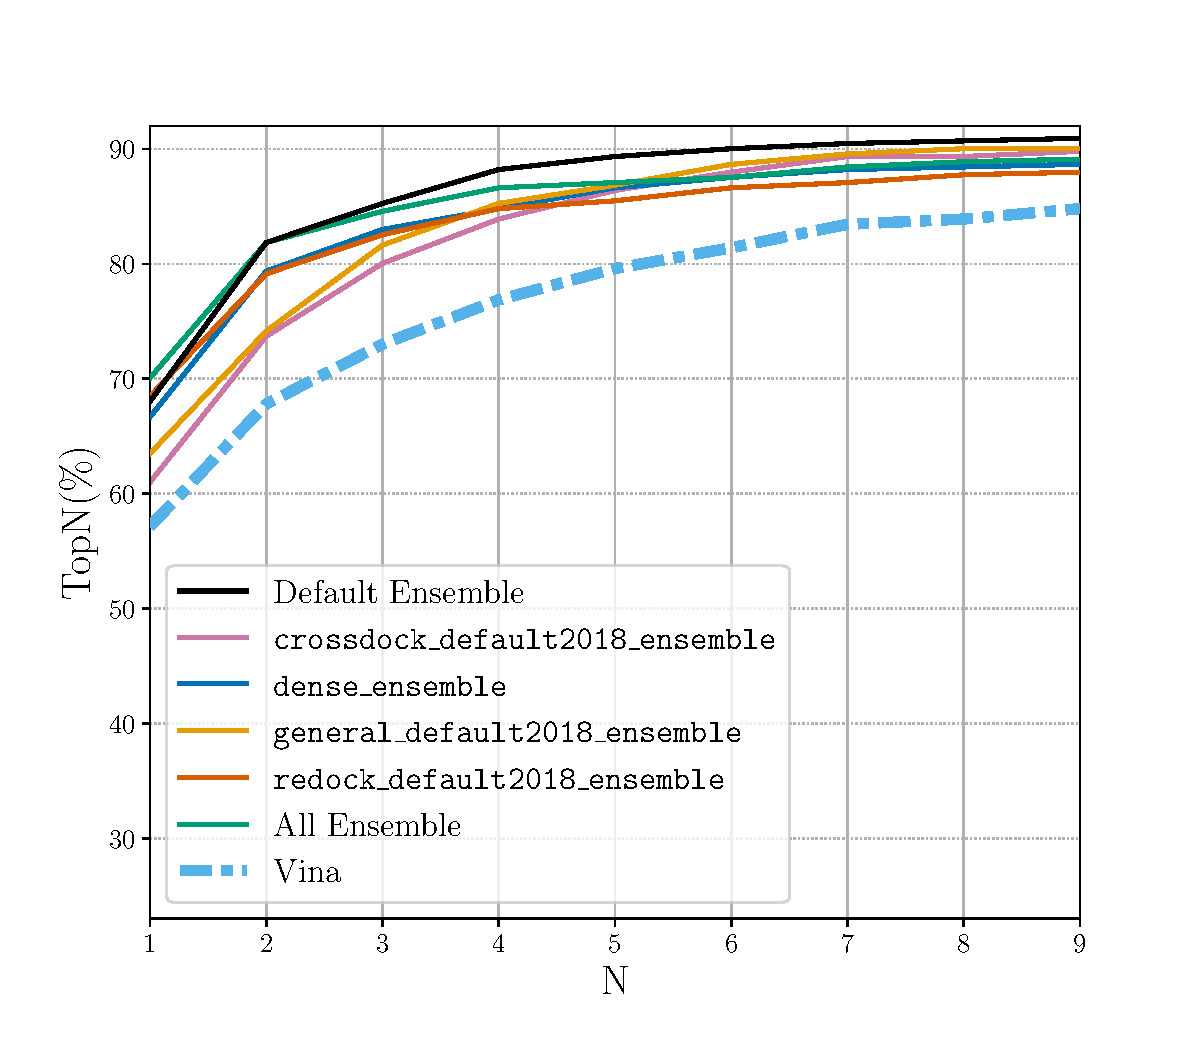
\includegraphics[width=\textwidth]{figures/redocking/ensemble_models_no2017_nocd2020_line.pdf}
		\caption{Redocking Ensembles}
		\label{fig:No2017NoCD20EnsRD}
        \end{subfigure}    
        \begin{subfigure}[b]{0.48\textwidth}    
		\centering
		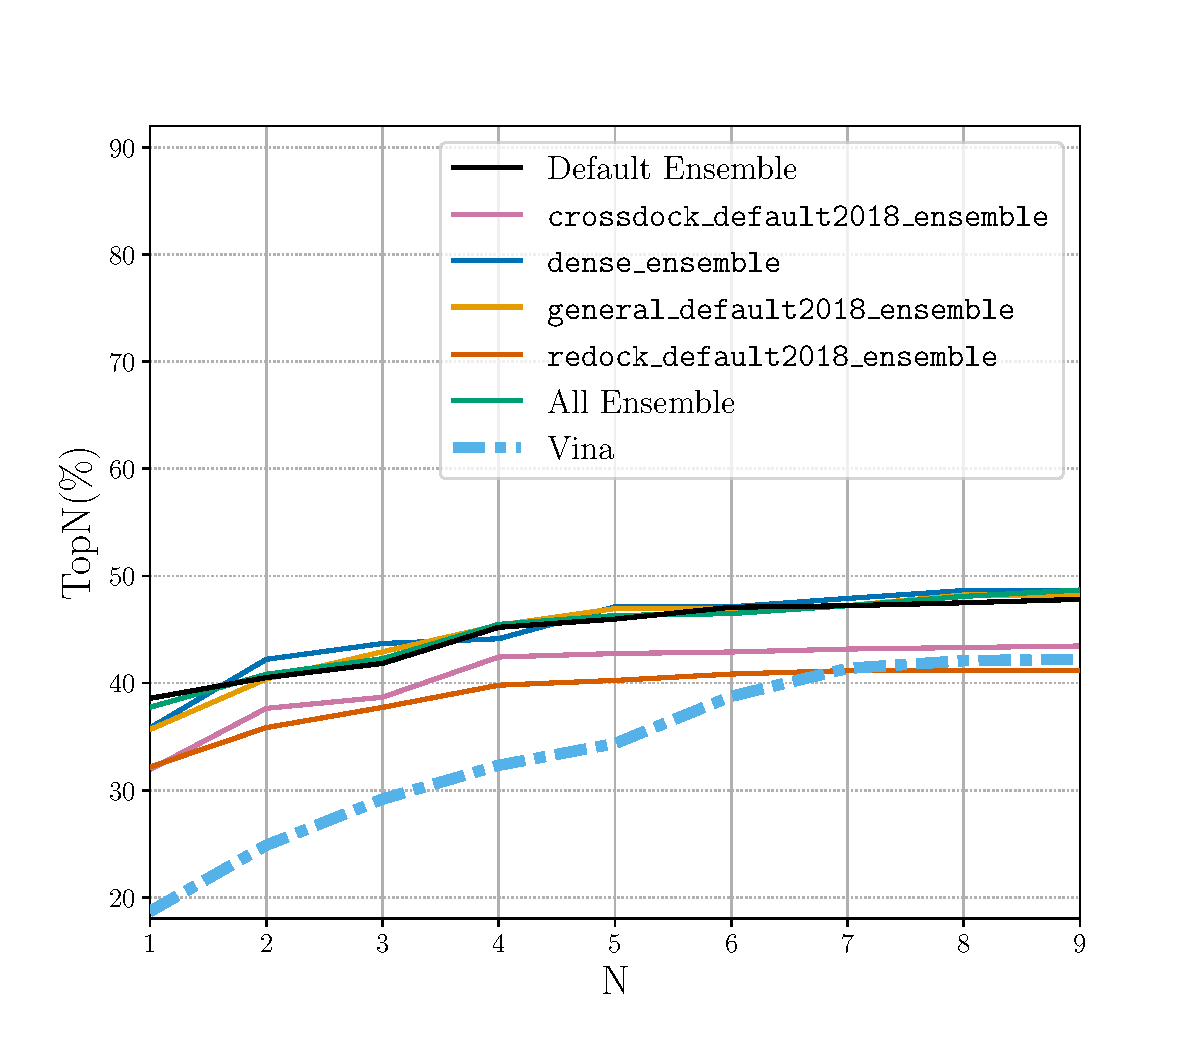
\includegraphics[width=\textwidth]{figures/crossdocking/ensemble_models_no2017_nocd2020_line.pdf}
		\caption{Crossdocking Ensembles}
                \label{fig:No2017NoCD20EnsCD}
        \end{subfigure}
	\caption{CNN model ensembles evaluated on the subset of systems not present in either the PDBbind general set v.2017 or the Crossdock2020 dataset. Ensemble models used with the default arguments defined above.}
	\label{fig:No2017NoCD20}
\end{figure}  

Finally, we examine the importance of the output CNNscore as a measure of the confidence of the prediction. 
\begin{figure}    
        \begin{subfigure}[b]{\textwidth}    
		\centering
		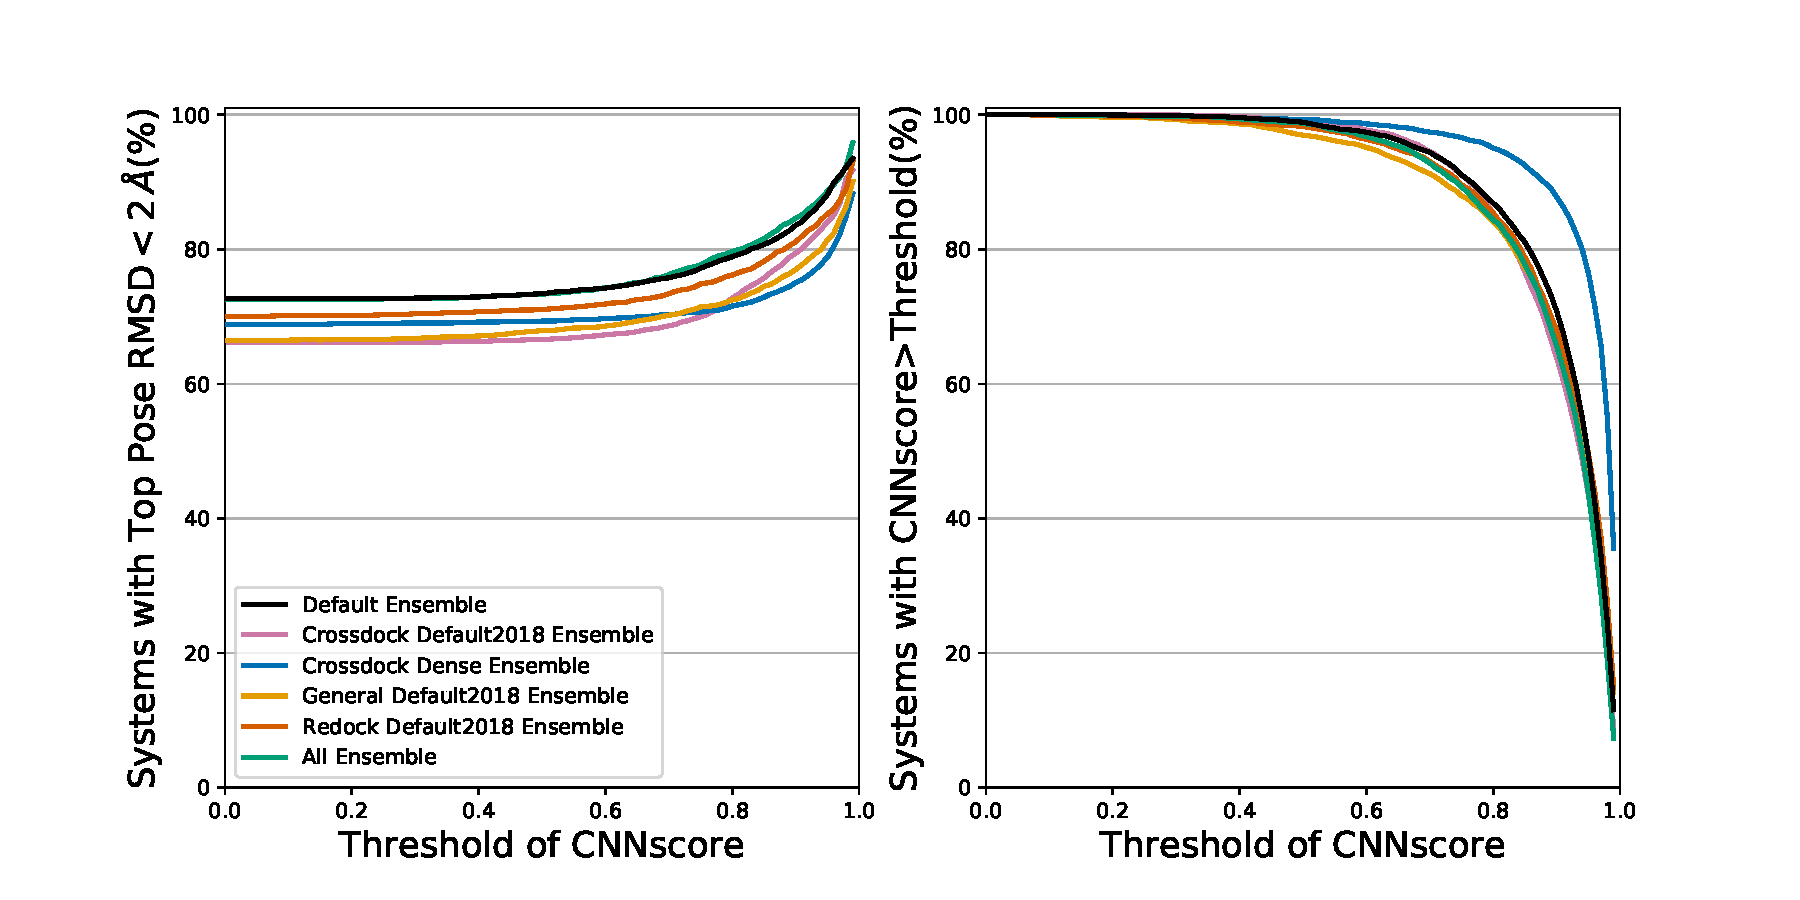
\includegraphics[width=\textwidth]{figures/redocking/thresh_cnnscore_ensembles.pdf}
		\caption{Redocking Ensembles}
		\label{fig:ThreshEnsRD}
        \end{subfigure}    
        \begin{subfigure}[b]{\textwidth}    
		\centering
		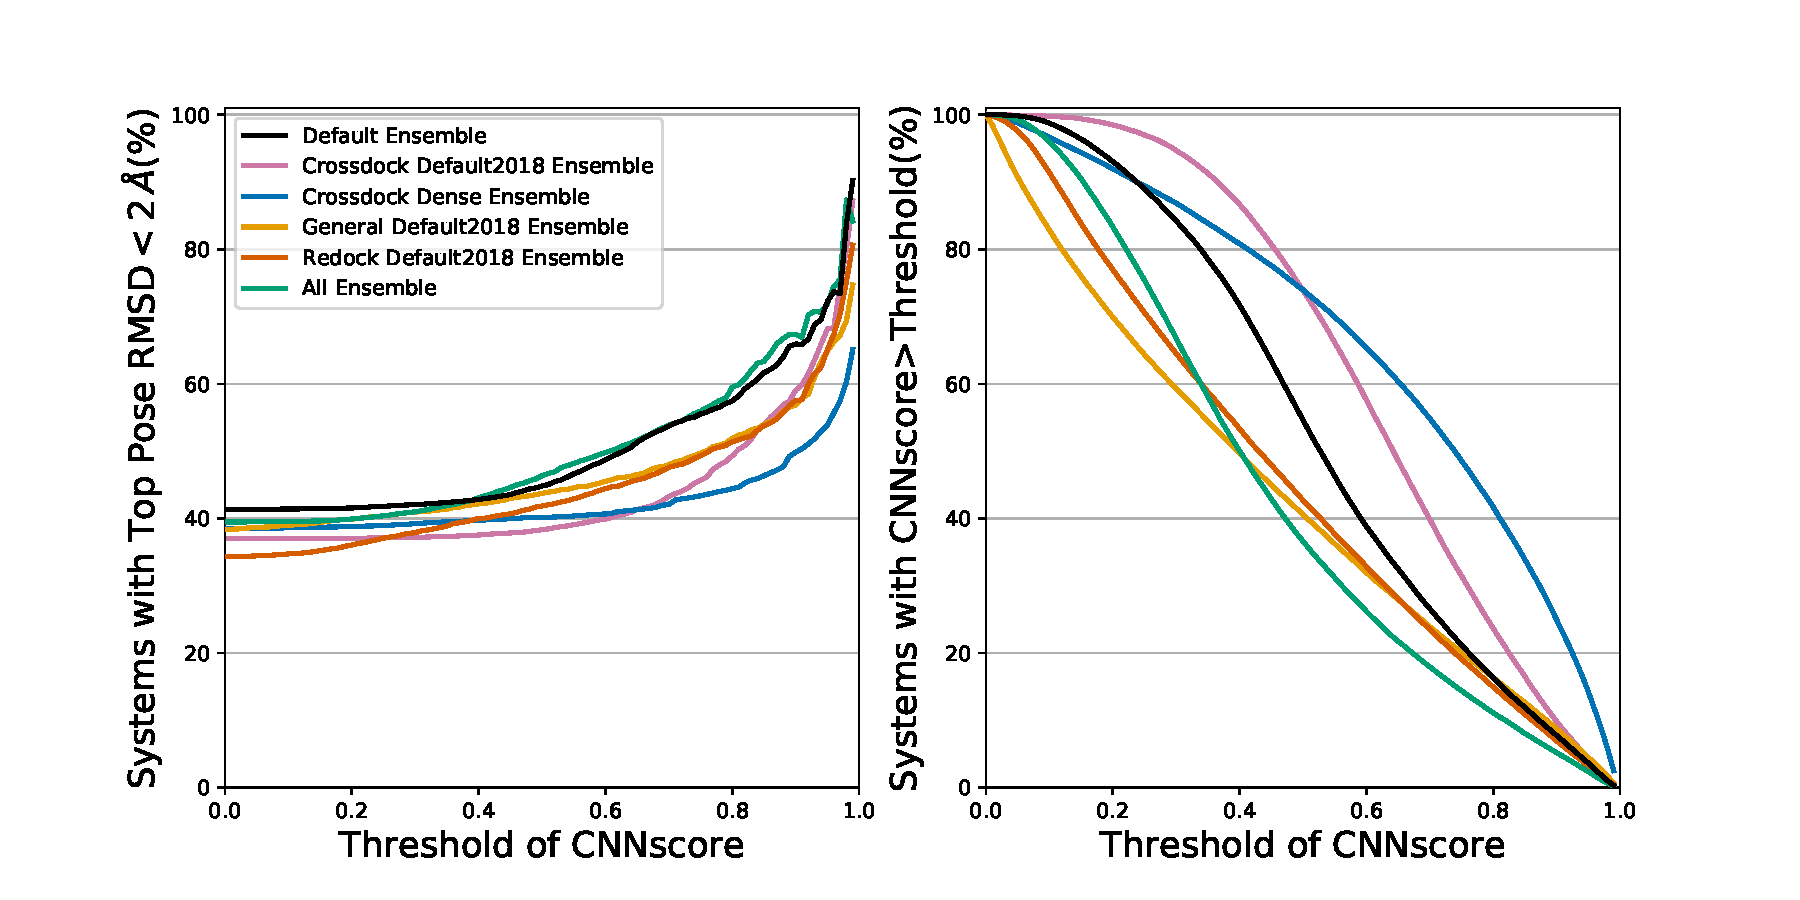
\includegraphics[width=\textwidth]{figures/crossdocking/thresh_cnnscore_ensembles.pdf}
		\caption{Crossdocking Ensembles}
                \label{fig:ThreshEnsCD}
        \end{subfigure}
	\caption{Thresholding the top pose by the score determined by the CNN}
	\label{fig:ScoreThresh}
\end{figure} 
We show in Figure~\ref{fig:ScoreThresh} that poses with high CNNscores are more likely to be low RMSD to the known binding pose. However, there when the CNNscore threshold is close to 1 each CNN ensemble has few poses remaining. Comparing the percentage of complexes remaining when thresholding by CNNscore, we can see that the CNN models are much more confident in the poses when they are performing the redocking task; at a threshold of 0.8 there are about 87\% remaining. All of the CNN ensembles score fewer poses with a high CNNscore for the crossdocking task; at a threshold of 0.8 there are about 16\% remaining. Though the same trend is true for crossdocking, that higher CNNscores imply a lower RMSD to the known crystal pose. Examining the crossdocking confidence, the Default Ensemble and All Ensemble both correctly score low RMSD poses with high CNNscores for about the same proportion of complexes, but if we examine the fraction of complexes remaining we see that the Default Ensemble has more complexes for a given threshold. The unique set of CNNs within the Default Ensemble are able to combine their knowledge of different types of ligand poses to correctly determine with high confidence when a pose is low RMSD to the binding pose.

\section{Discussion}
We show that our computational docking software \textsc{Gnina} is able to outperform AutoDock Vina by using CNN models to rescore generated poses. Without using a CNN model, our software is equivalent to using the \textsc{Smina} docking software, which is a fork of Vina. \textsc{Gnina} allows the user to utilize CNN models as scoring functions within the docking pipeline in a variety of ways. The various CNN scoring options allow the specified CNN models to replace the scoring function in the sampling, refinement, and rescoring steps of the docking pipeline. We first establish an ensemble of built-in CNN models to be used as the default ensemble. This ensemble of models is selected for its high docking performance and quick run-time. The selected ensemble, termed the Default Ensemble, is able to exceed the ranking performance of Vina while only adding two seconds to the average compute time when utilizing GPUs. The Default Ensemble performs almost equally well when performing refinement of the sampled poses rather than using the Vina scoring function. Refinement with the CNN models is not recommended as the compute cost is significant and the performance is less than simply using the CNN models to rescore the poses refined by the Vina scoring function.

We next derive the default parameters when using the Default Ensemble for docking with \textsc{Gnina}. \texttt{autobox\_add} increases the amount of space around the defined binding pocket to allow more volume for the sampling to investigate. Increases in \texttt{autobox\_add} decrease the accuracy of the predicted binding pose when the binding pocket is known. We find that increases in \texttt{exhaustiveness}, or the number of Monte Carlo chains run, boost the performance of the docking procedure at the cost of extra computation. Similarly, increasing the number of poses saved from each Monte Carlo chain, \texttt{num\_mc\_saved}, and the number of poses output by the docking pipeline, \texttt{num\_modes}, increase the performance of the docking routine at the expense of increased computation. The value of the \texttt{cnn\_rotation} and the value of \texttt{min\_rmsd\_filter} do not seem to alter the performance of the docking pipeline. The default arguments for when the binding pocket is explicitly defined are set as such for \textsc{Gnina}; \texttt{autobox\_add} (4), \texttt{exhaustiveness} (8), \texttt{num\_mc\_saved} (50), \texttt{num\_modes} (9), \texttt{min\_rmsd\_filter} (1.0), and \texttt{cnn\_rotation} (0). However, when the exact binding pocket is not known and the whole protein is used as the ``defined'' binding pocket we see that \texttt{exhaustiveness} has a much greater impact on performance. When performing whole protein docking, we therefore recommend that the largest value of \texttt{exhaustiveness} that can be used given time constraints.

Finally, we probe the performance of the CNN ensembles at scoring ligand conformations. In order to ensure that our CNN models are generalizing to unseen protein-ligand complexes we filter the redocking and crossdocking benchmark datasets to only include protein-ligand pairs that were not seen during training of the CNNs. On both subsets of the data, we show that our CNN model ensembles are able to outperform the Vina scoring function. The CNN models are able to generalize to unseen examples and properly score the ligand conformations such that the low RMSD poses are ranked higher more often than when using the Vina scoring function. The score output can provide a probability of a pose being less than 2 \AA~from the binding pose. When the CNN score outputs a score greater than 0.8 there is at least a 57\% probability that the pose has less than 2 \AA~RMSD from the binding pose, even when crossdocking. The score output by the CNN models can be used as an indicator of the confidence in the quality of the generated ligand conformation.

The source code and a pre-built docker container for Gnina is available under the Apache License, Version 2.0 from \url{https://github.com/gnina/gnina}.


\begin{acknowledgement}
The authors thank  for their sagacious contributions during the preparation of this manuscript.
This work is supported by R01GM108340 from the National Institute of General Medical Sciences and is supported in part by the University of Pittsburgh Center for Research Computing through the resources provided.



\end{acknowledgement}

%%%%%%%%%%%%%%%%%%%%%%%%%%%%%%%%%%%%%%%%%%%%%%%%%%%%%%%%%%%%%%%%%%%%%
%% The same is true for Supporting Information, which should use the
%% suppinfo environment.
%%%%%%%%%%%%%%%%%%%%%%%%%%%%%%%%%%%%%%%%%%%%%%%%%%%%%%%%%%%%%%%%%%%%%
\begin{suppinfo}
  


\end{suppinfo}

%%%%%%%%%%%%%%%%%%%%%%%%%%%%%%%%%%%%%%%%%%%%%%%%%%%%%%%%%%%%%%%%%%%%%
%% The appropriate \bibliography command should be placed here.
%% Notice that the class file automatically sets \bibliographystyle
%% and also names the section correctly.
%%%%%%%%%%%%%%%%%%%%%%%%%%%%%%%%%%%%%%%%%%%%%%%%%%%%%%%%%%%%%%%%%%%%%
\bibliography{references}

\end{document}
